%%%%%%%%%%%%%%%%%%%%%%%%%%%%%%%%%%%%%%%%%
% Sullivan Business Report
% LaTeX Template
% Version 1.0 (May 5, 2022)
%
% This template originates from:
% https://www.LaTeXTemplates.com
%
% Author:
% Vel (vel@latextemplates.com)
%
% License:
% CC BY-NC-SA 4.0 (https://creativecommons.org/licenses/by-nc-sa/4.0/)
%
%%%%%%%%%%%%%%%%%%%%%%%%%%%%%%%%%%%%%%%%%


%----------------------------------------------------------------------------------------
%	CLASS, PACKAGES AND OTHER DOCUMENT CONFIGURATIONS
%----------------------------------------------------------------------------------------

\documentclass[
    a4paper, % Paper size, use either a4paper or letterpaper
	12pt, % Default font size, the template is designed to look good at 12pt so it's best not to change this
	%unnumberedsections, % Uncomment for no section numbering
    ]{CSSullivanBusinessReport}
    
    \addbibresource{sample.bib} % BibLaTeX bibliography file

%----------------------------------------------------------------------------------------
%	REPORT INFORMATION
%----------------------------------------------------------------------------------------

\reporttitle{CPE 233 Hardware Assignment 3} % The report title is to appear on the title page and page headers, do not create manual new lines here as this will carry over to page headers

\reportsubtitle{Register File and Verification} % Report subtitle, include new lines if needed

\reportauthors{Report by:\\\smallskip Ethan Vosburg (evosburg@calpoly.edu)} % Report authors/group/department, include new lines if needed

\reportdate{\today} % Report date, include new lines for additional information if needed

\rightheadercontent{
\includegraphics[width=3cm]{creodocs_logo.pdf}} % The content in the right header, you may want to add your own company logo or use your company/department name or leave this command empty for no right header content

%----------------------------------------------------------------------------------------

\begin{document}

%----------------------------------------------------------------------------------------
%	TITLE PAGE
%----------------------------------------------------------------------------------------

\thispagestyle{empty} % Suppress headers and footers on this page

\begin{fullwidth} % Use the whole page width
	\vspace*{-0.075\textheight} % Pull logo into the top margin
	
	\hfill
\includegraphics[width=5cm]{creodocs_logo.pdf} % Company logo

	\vspace{0.15\textheight} % Vertical whitespace

	\parbox{0.9\fulltextwidth}{\fontsize{50pt}{52pt}\selectfont\raggedright\textbf{\reporttitle}\par} % Report title, intentionally at less than full width for nice wrapping. Adjust the width of the \parbox and the font size as needed for your title to look good.
	
	\vspace{0.03\textheight} % Vertical whitespace
	
	{\LARGE\textit{\textbf{\reportsubtitle}}\par} % Subtitle
	
	\vfill % Vertical whitespace
	
	{\Large\reportauthors\par} % Report authors, group or department
	
	\vfill\vfill\vfill % Vertical whitespace
	
	{\large\reportdate\par} % Report date
\end{fullwidth}

\newpage

%----------------------------------------------------------------------------------------
%	DISCLAIMER/COPYRIGHT PAGE
%----------------------------------------------------------------------------------------

% \thispagestyle{empty} % Suppress headers and footers on this page

% \begin{twothirdswidth} % Content in this environment to be at two-thirds of the whole page width
% 	\footnotesize % Reduce font size
	
% 	\subsection*{Disclaimer}

% 	Lorem ipsum dolor sit amet, consectetur adipiscing elit. Praesent porttitor arcu luctus, imperdiet urna iaculis, mattis eros. Pellentesque iaculis odio vel nisl ullamcorper, nec faucibus ipsum molestie. Sed dictum nisl non aliquet porttitor. Etiam vulputate arcu dignissim, finibus sem et, viverra nisl. Aenean luctus congue massa, ut laoreet metus ornare in. Nunc fermentum nisi imperdiet lectus tincidunt vestibulum at ac elit.
	
% 	\subsection*{Copyright}
	
% 	\textcopyright~[Year] [Company] 
	
% 	Copyright notice text\ldots In hac habitasse platea dictumst. Curabitur mattis elit sit amet justo luctus vestibulum. In hac habitasse platea dictumst. Pellentesque lobortis justo enim, a condimentum massa tempor eu. Ut quis nulla a quam pretium eleifend nec eu nisl. Nam cursus porttitor eros, sed luctus ligula convallis quis.
	
% 	\subsection*{Contact}
	
% 	Address Line 1\\
% 	Address Line 2\\
% 	Address Line 3
	
% 	Business Number 123456
	
% 	Contact: name@company.com
	
% 	\vfill % Push the following down to the bottom of the page
	
% 	\subsubsection*{Changelog}
	
% 	\scriptsize % Reduce font size further
	
% 	\begin{tabular}{@{} L{0.05\linewidth} L{0.15\linewidth} L{0.6\linewidth} @{}} % Column widths specified here, change as needed for your content
% 		\toprule
% 		v1.0 & 20XX-02-05 & Lorem ipsum dolor sit amet, consectetur adipiscing elit. Praesent porttitor arcu luctus, imperdiet urna iaculis, mattis eros.\\
% 		v1.1 & 20XX-02-27 & Pellentesque iaculis odio vel nisl ullamcorper, nec faucibus ipsum molestie.\\
% 		v1.2 & 20XX-03-15 & Sed dictum nisl non aliquet porttitor.\\
% 		\bottomrule
% 	\end{tabular}
% \end{twothirdswidth}

% \newpage

%----------------------------------------------------------------------------------------
%	TABLE OF CONTENTS
%----------------------------------------------------------------------------------------
\bigskip
\begin{twothirdswidth} % Content in this environment to be at two-thirds of the whole page width
	\tableofcontents % Output the table of contents, automatically generated from the section commands used in the document
\end{twothirdswidth}

\newpage

%----------------------------------------------------------------------------------------
%	SECTIONS
%----------------------------------------------------------------------------------------
\begin{fullwidth} % Use the whole page width

\section{Project Description} % Top level section

In this project, a register file was created and tested using a testbench. The testbench was able to verify that the register file worked properly and passed all of the test cases. The register file was able to take in two different addresses and return the correct information as well as take in one address and write to a specific address.


\section{Structural Design} % Second level section

\subsection{Overall Elaborated Design} % Third level section

\begin{figure}[H]
    \centering
    \captionsetup{style=widetable}
    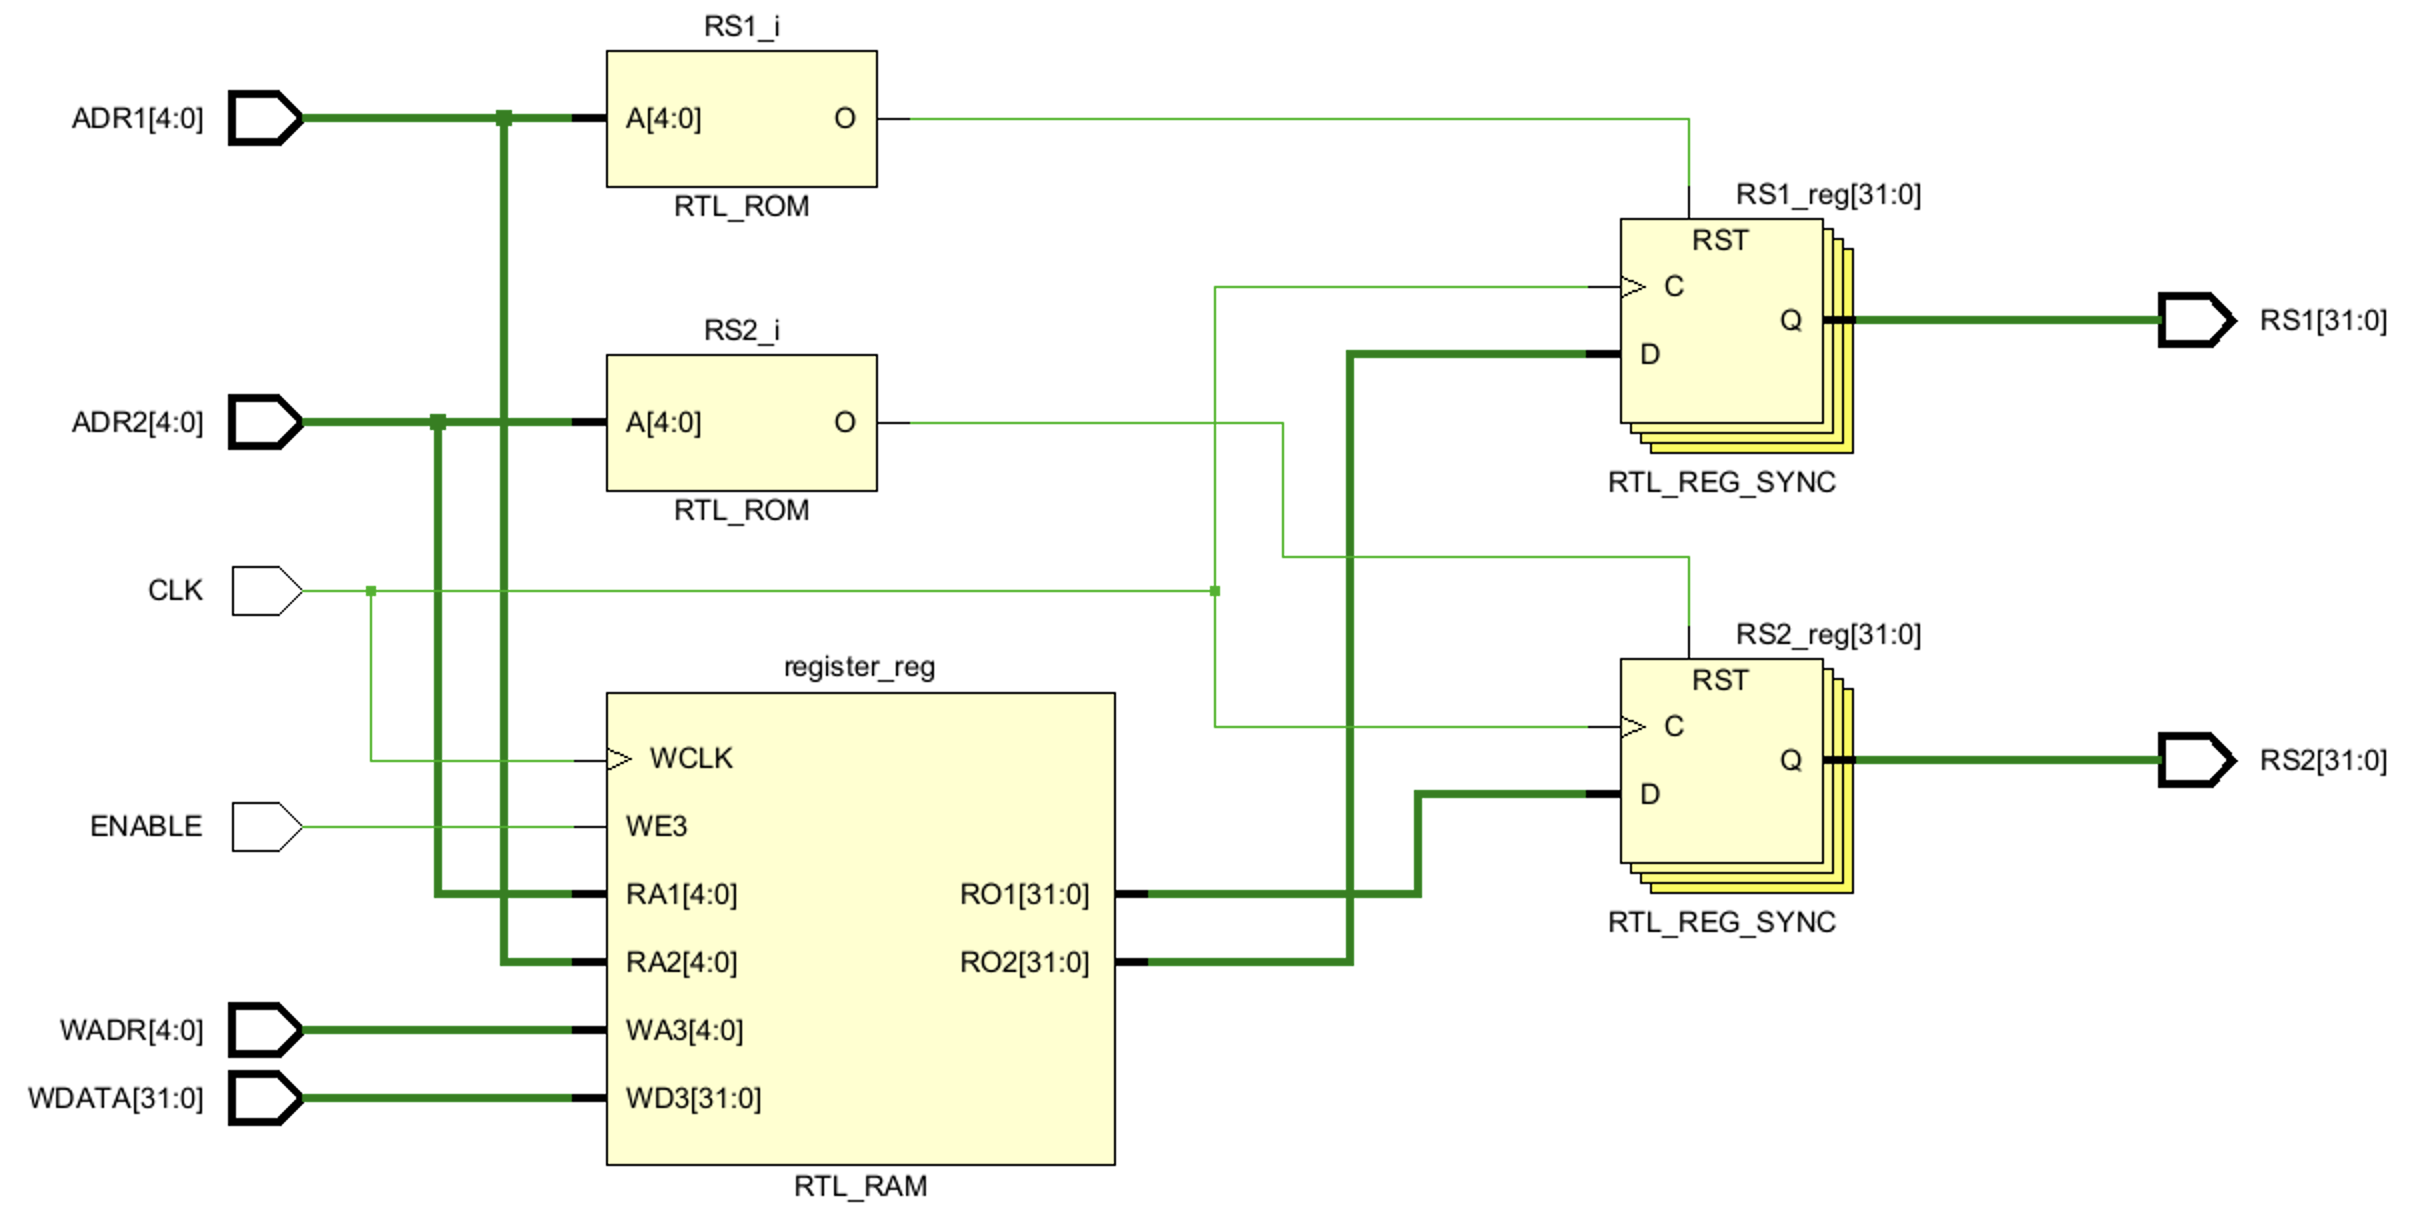
\includegraphics[width=.80\pdfpagewidth]{Figures/RegFile Elaborated Design.png}
    \caption{Program Counter Elaborated Design}
    \label{fig:PCElaboratedDesign}
\end{figure}


\section{Synthesis Warnings} % Second level section

\begin{figure}[H]
    \captionsetup{style=widetable}
    \makebox[.80\pdfpagewidth]{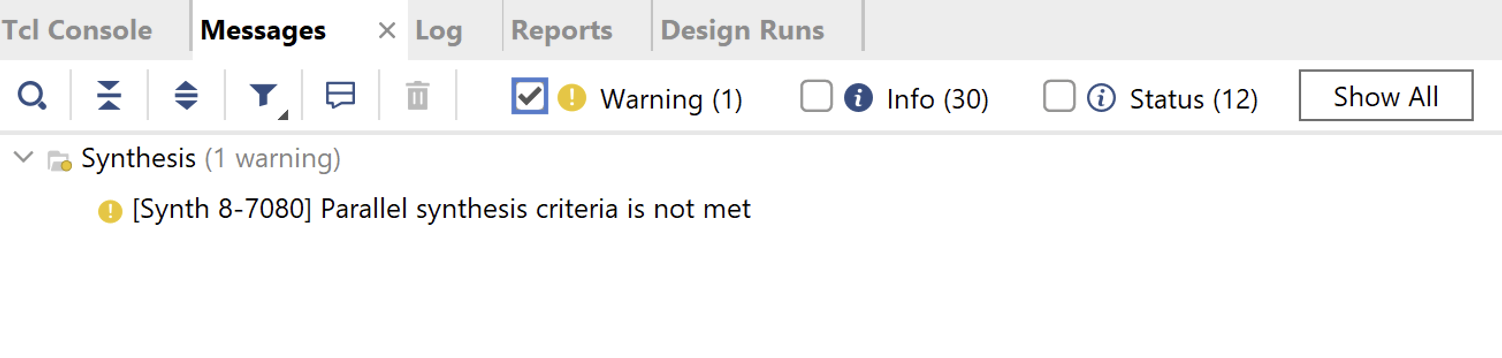
\includegraphics[width=.75\pdfpagewidth]{Figures/Program Counter Console Warnings.png}}
    \caption{Synthesis Warnings}
    \label{fig:SynthesisWarnings}
\end{figure}

\section{Verification} % Second level section

\subsection{Testbench Coverage} % Third level section

When testing this design, there were several test cases that were used to verify that the design was working properly. The test cases are listed below.

\begin{enumerate}
    \item \textbf{Random Bits Test:} This test case was used to verify that the RegFile could store any random number in all of the registers and then provide that number through both of the register outputs.
    \item \textbf{Zero Bits Test:} This test case was used to verify that the RegFile could store a zero in all of the registers and then provide that number through both of the register outputs.
    \item \textbf{Enable Write Test:} This test case was used to verify that the enable write bit would allow the RegFile to write to the registers when it was high and not write to the registers when it was low.
    \item \textbf{Min Bits Test:} This test case was used to verify that the RegFile could store the minimum number in all of the registers and then provide that number through both of the register outputs.
    \item \textbf{Max Bits Test:} This test case was used to verify that the RegFile could store the maximum number in all of the registers and then provide that number through both of the register outputs.
\end{enumerate}

\captionsetup{style=widetable}
\subsection{Testbench Code} % Third level section

\lstinputlisting[language=Verilog, caption=Verilog Testbench for Program Counter]{/Users/ethanvosburg/Documents/git/CPE-233-Otter/HW3-RegFile/RegFile/RegFile.srcs/sim_1/new/RegFile_TB.sv}

\newpage
\subsection{Testbench Output} % Third level section
Running this testbench produced the following output in the TCL code console:

\begin{lstlisting}[language=Verilog, caption=TCl Output from ProgramCounterEnv\_TB]
----------------------------------------

RegFile Testbench

----------------------------------------

Setup Complete
Random Bits Test Passed
Zero Bits Test Passed
Enable Write Test Passed
Min Bits Test Passed
Max Bits Test Passed
----------------------------------------

OVERALL PASS

----------------------------------------

$finish called at time : 3980 ns
\end{lstlisting}

\newpage
\subsection{Simulation Results} % Third level section

Running this testbench produced the following simulation results:

\begin{figure}[H]
    \centering
    \captionsetup{style=widetable}
    \makebox[.80\pdfpagewidth]{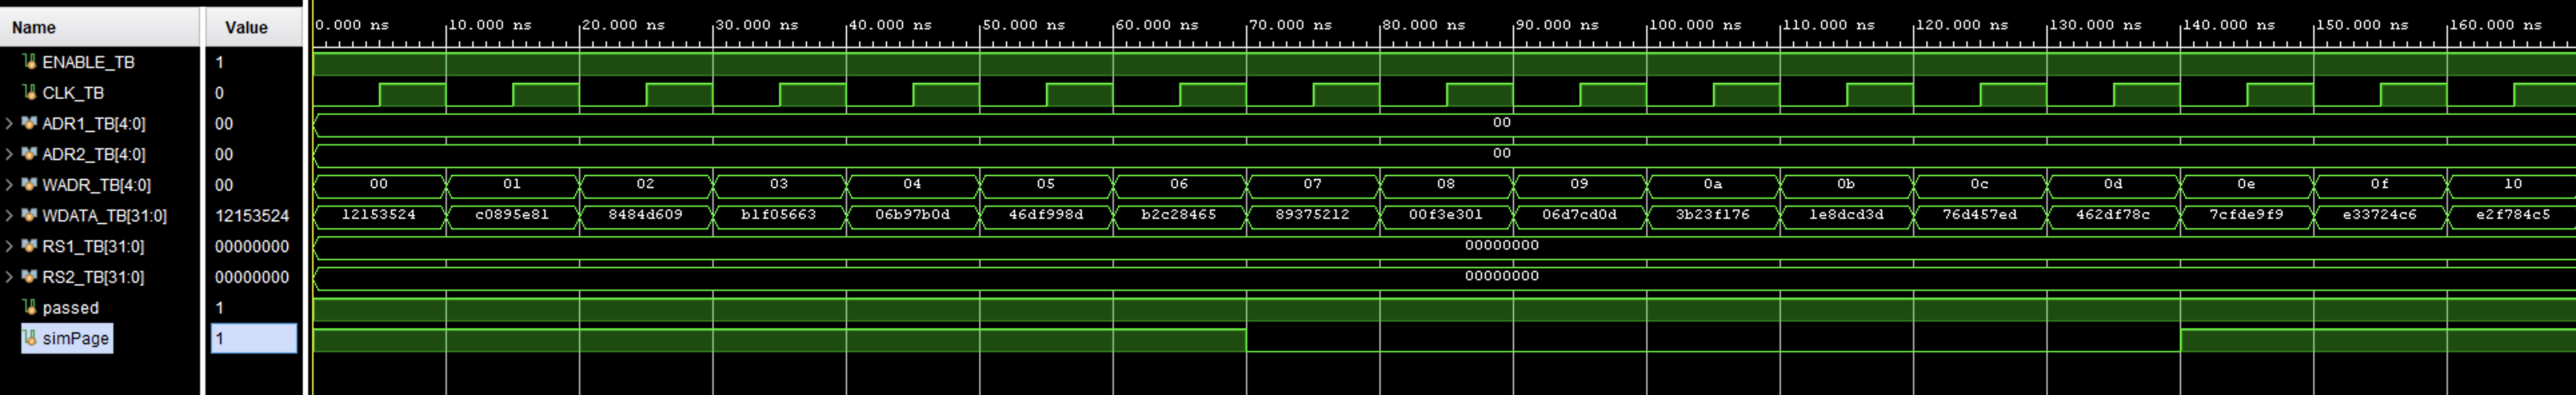
\includegraphics[width=.8\pdfpagewidth]{Figures/RegFile Simulation 00.png}}
    \caption{RegFile Simulation 0ns - 140ns}
    \label{fig:regfilesim1}
\end{figure}

\begin{figure}[H]
    \centering
    \captionsetup{style=widetable}
    \makebox[.80\pdfpagewidth]{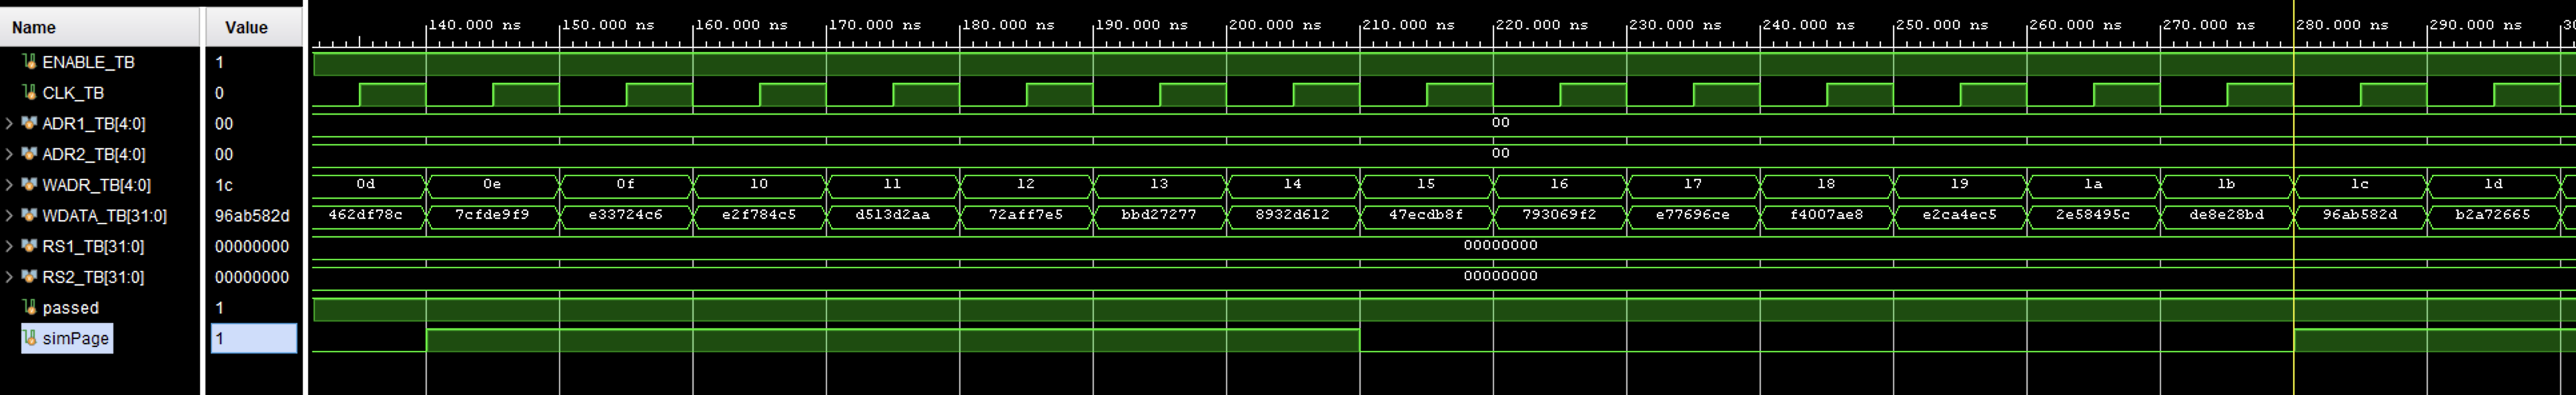
\includegraphics[width=.8\pdfpagewidth]{Figures/RegFile Simulation 01.png}}
    \caption{RegFile Simulation 140ns - 280ns}
    \label{fig:regfilesim2}
\end{figure}

\begin{figure}[H]
    \centering
    \captionsetup{style=widetable}
    \makebox[.80\pdfpagewidth]{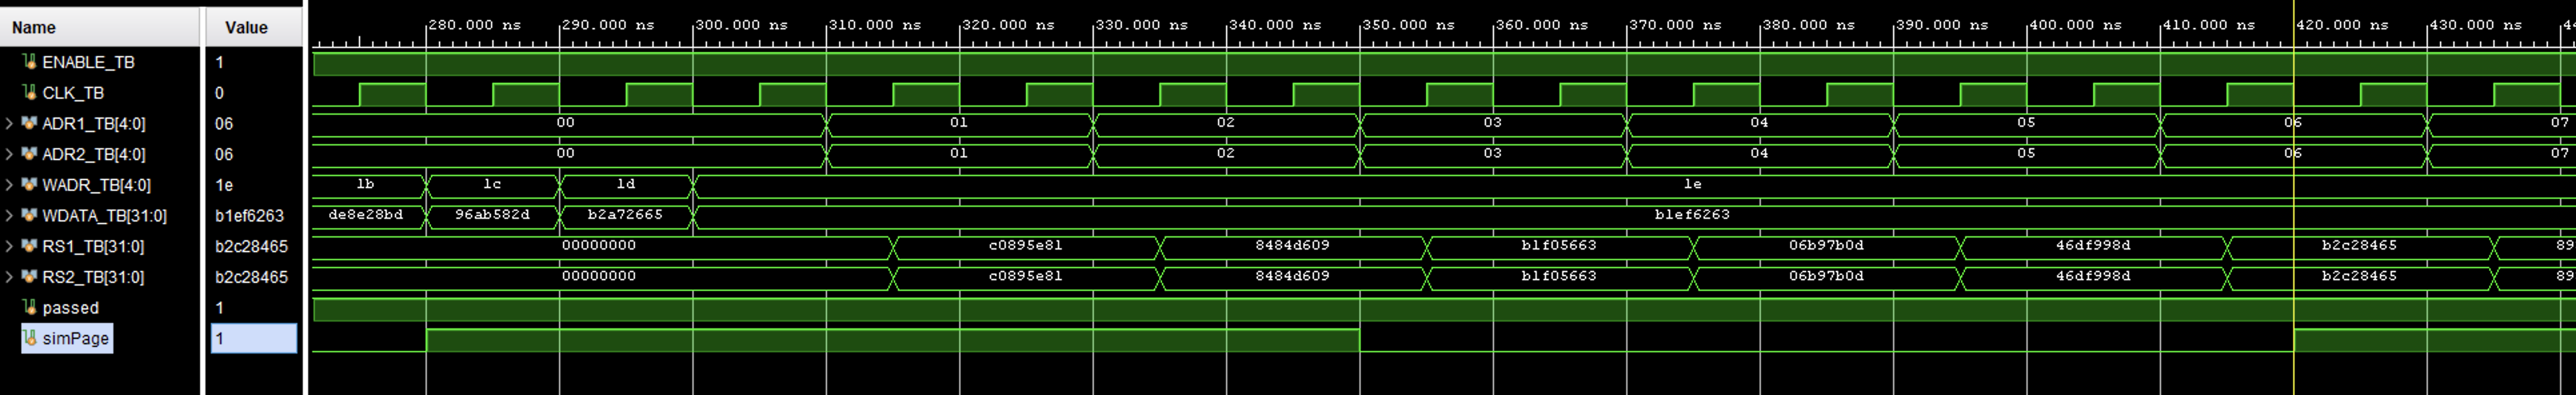
\includegraphics[width=.8\pdfpagewidth]{Figures/RegFile Simulation 02.png}}
    \caption{RegFile Simulation 280ns - 420ns}
    \label{fig:regfilesim3}
\end{figure}

\begin{figure}[H]
    \centering
    \captionsetup{style=widetable}
    \makebox[.80\pdfpagewidth]{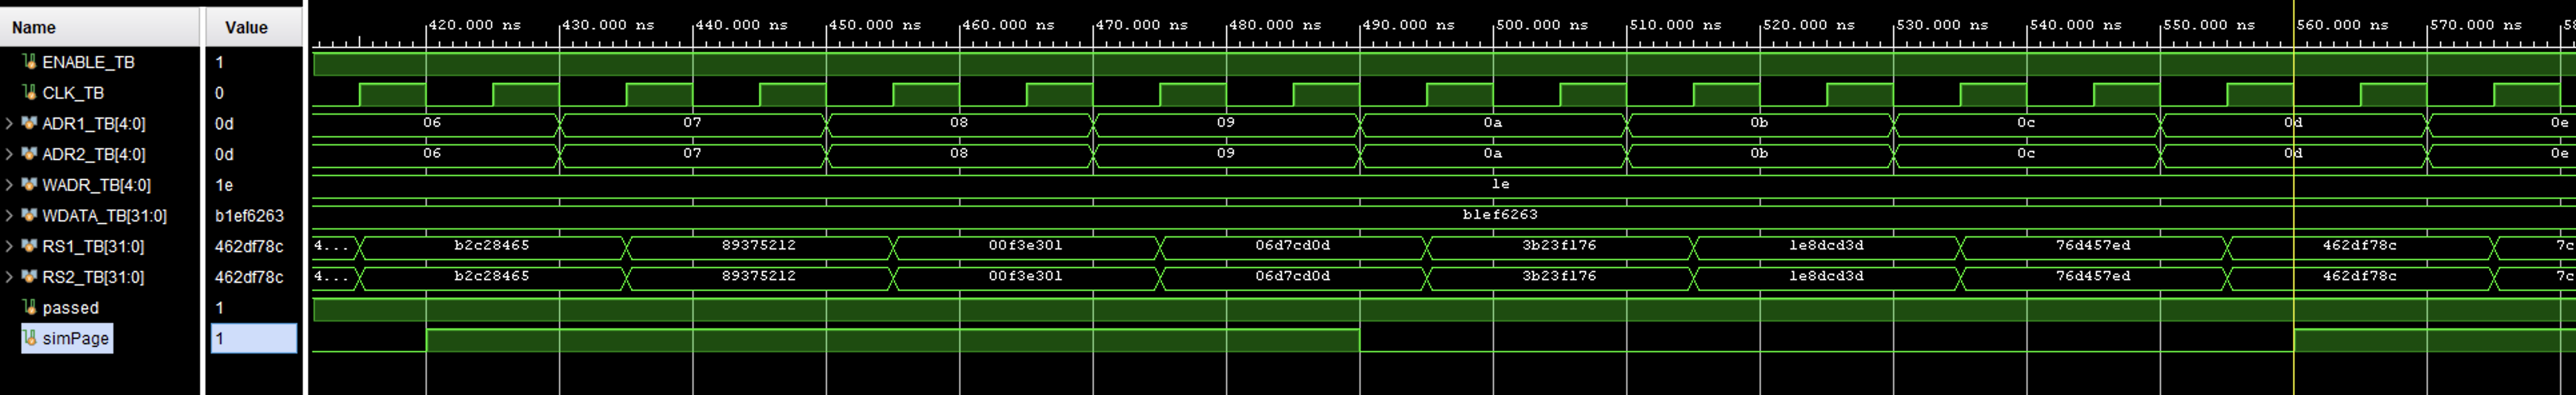
\includegraphics[width=.8\pdfpagewidth]{Figures/RegFile Simulation 03.png}}
    \caption{RegFile Simulation 420ns - 560ns}
    \label{fig:regfilesim4}
\end{figure}

\begin{figure}[H]
    \centering
    \captionsetup{style=widetable}
    \makebox[.80\pdfpagewidth]{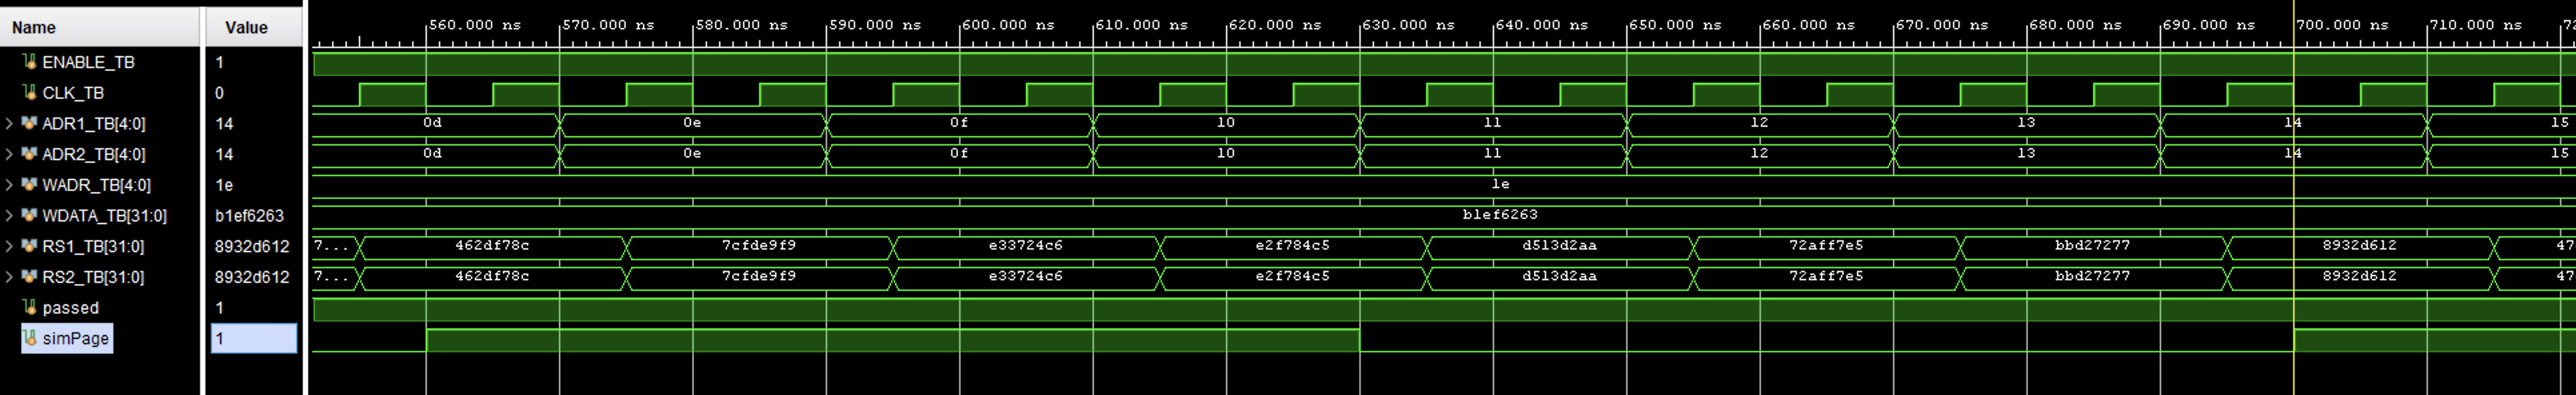
\includegraphics[width=.8\pdfpagewidth]{Figures/RegFile Simulation 04.png}}
    \caption{RegFile Simulation 560ns - 700ns}
    \label{fig:regfilesim5}
\end{figure}

\begin{figure}[H]
    \centering
    \captionsetup{style=widetable}
    \makebox[.80\pdfpagewidth]{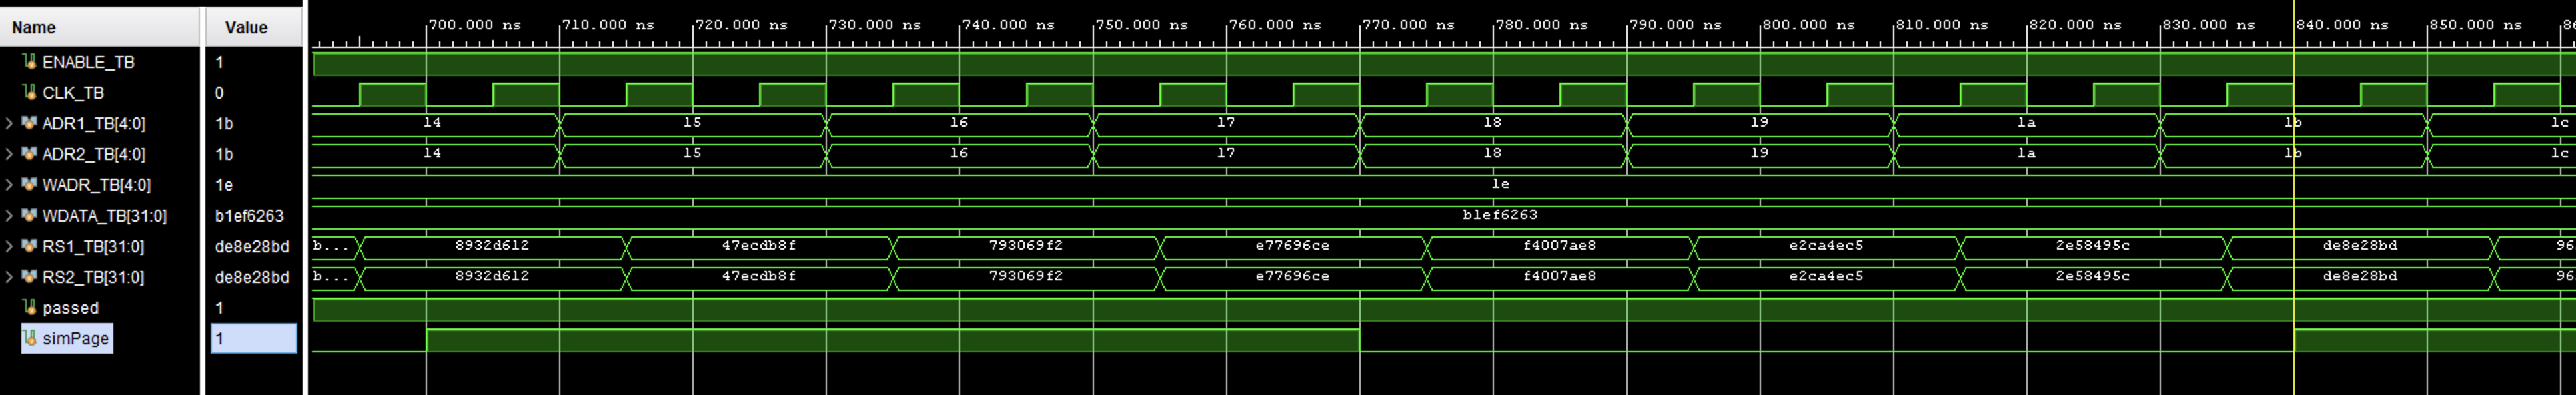
\includegraphics[width=.8\pdfpagewidth]{Figures/RegFile Simulation 05.png}}
    \caption{RegFile Simulation 700ns - 840ns}
    \label{fig:regfilesim6}
\end{figure}

\begin{figure}[H]
    \centering
    \captionsetup{style=widetable}
    \makebox[.80\pdfpagewidth]{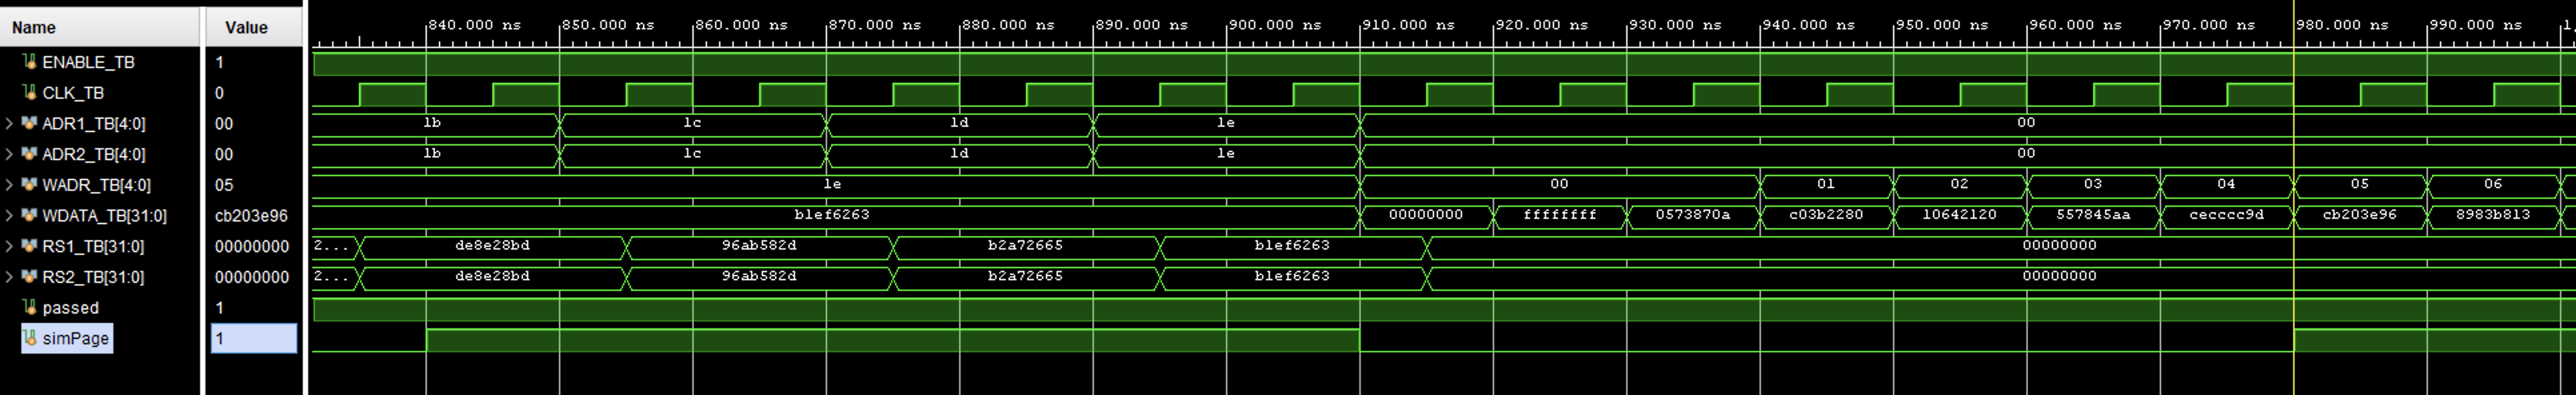
\includegraphics[width=.8\pdfpagewidth]{Figures/RegFile Simulation 06.png}}
    \caption{RegFile Simulation 840ns - 980ns}
    \label{fig:regfilesim7}
\end{figure}

\begin{figure}[H]
    \centering
    \captionsetup{style=widetable}
    \makebox[.80\pdfpagewidth]{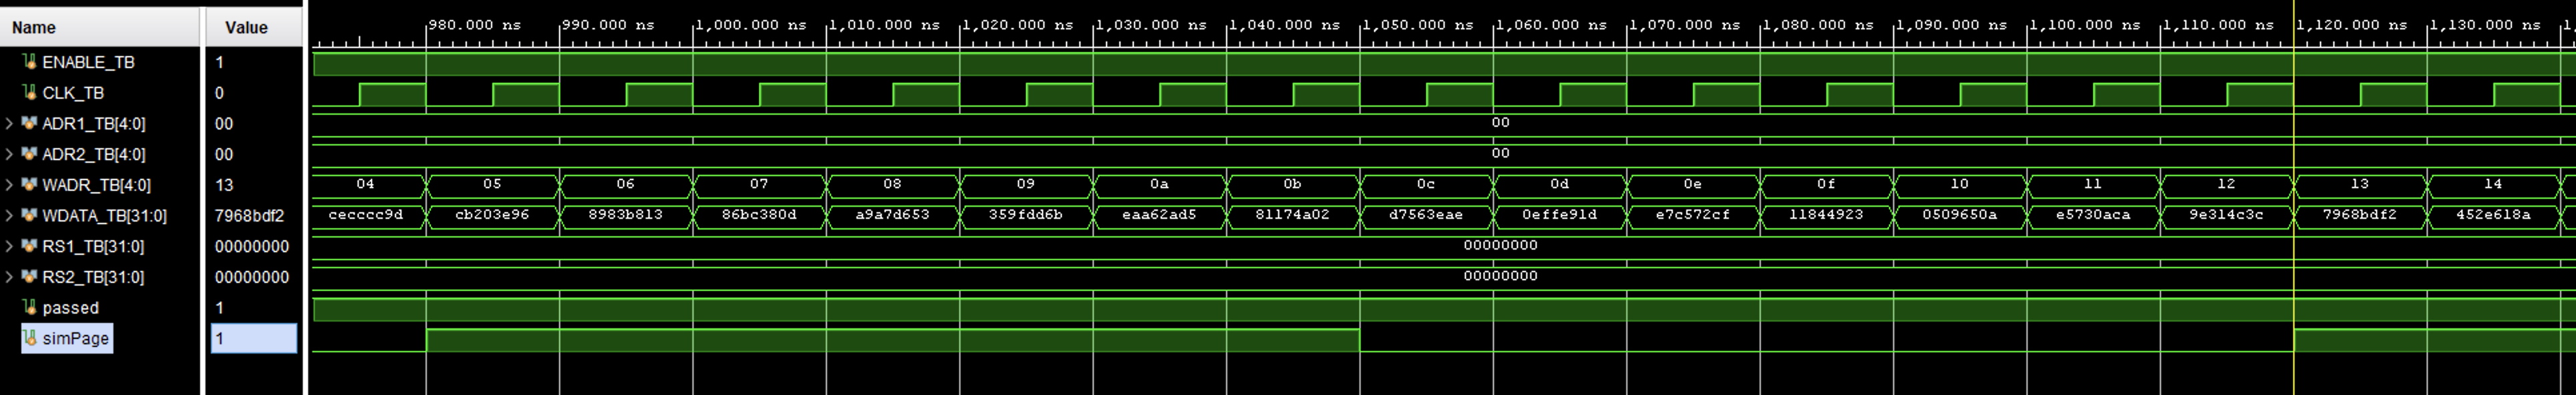
\includegraphics[width=.8\pdfpagewidth]{Figures/RegFile Simulation 07.png}}
    \caption{RegFile Simulation 980ns - 1120ns}
    \label{fig:regfilesim8}
\end{figure}

\begin{figure}[H]
    \centering
    \captionsetup{style=widetable}
    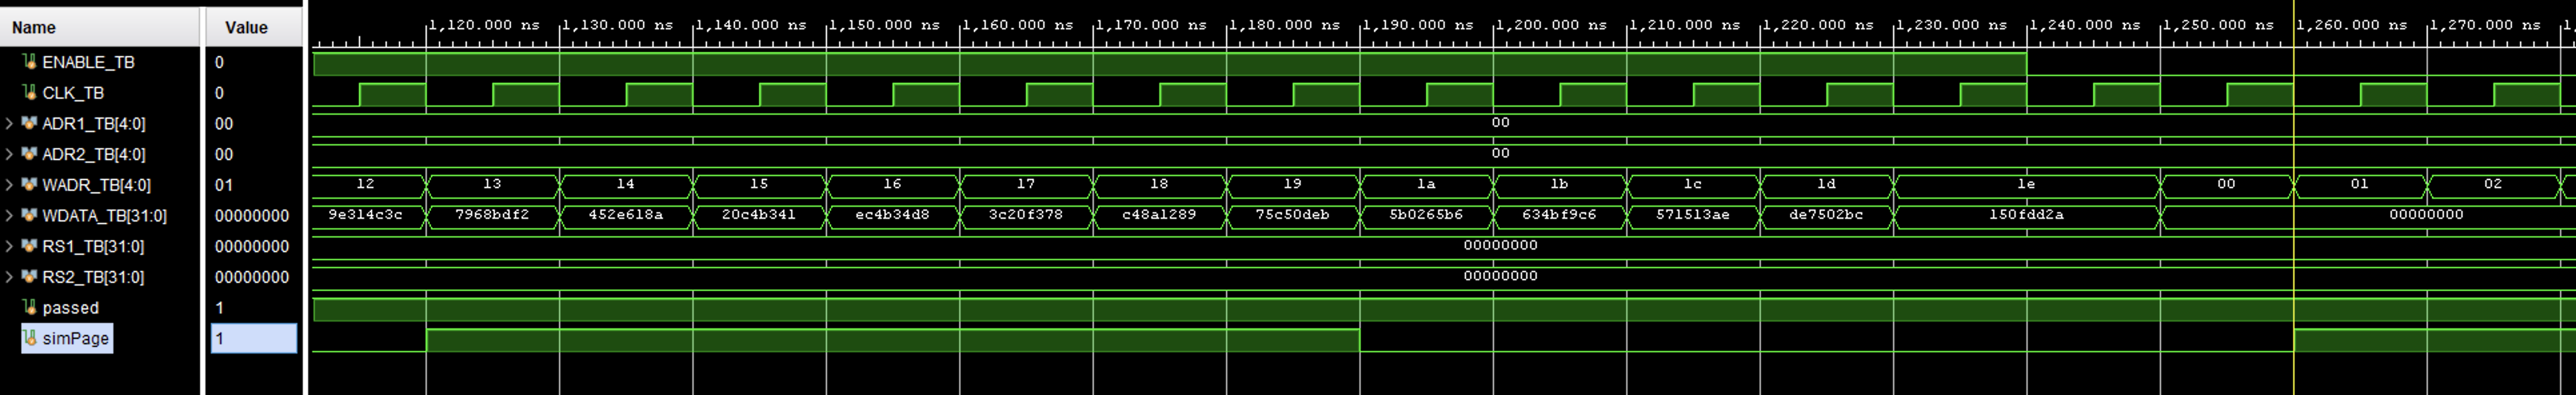
\includegraphics[width=.80\pdfpagewidth]{Figures/RegFile Simulation 08.png}
    \caption{RegFile Simulation 1120ns - 1260ns}
    \label{fig:regfilesim9}
\end{figure}

\begin{figure}[H]
    \centering
    \captionsetup{style=widetable}
    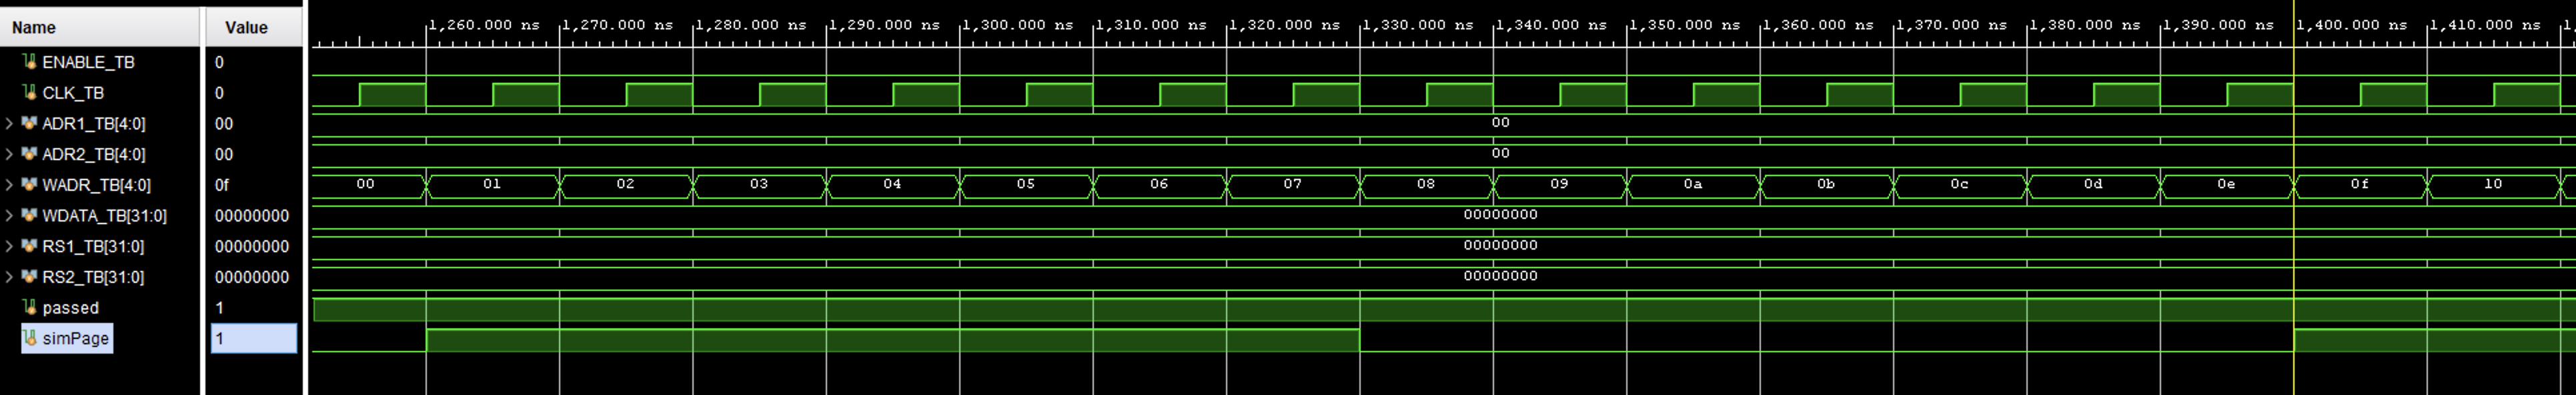
\includegraphics[width=.80\pdfpagewidth]{Figures/RegFile Simulation 09.png}
    \caption{RegFile Simulation 1260ns - 1400ns}
    \label{fig:regfilesim10}
\end{figure}

\begin{figure}[H]
    \centering
    \captionsetup{style=widetable}
    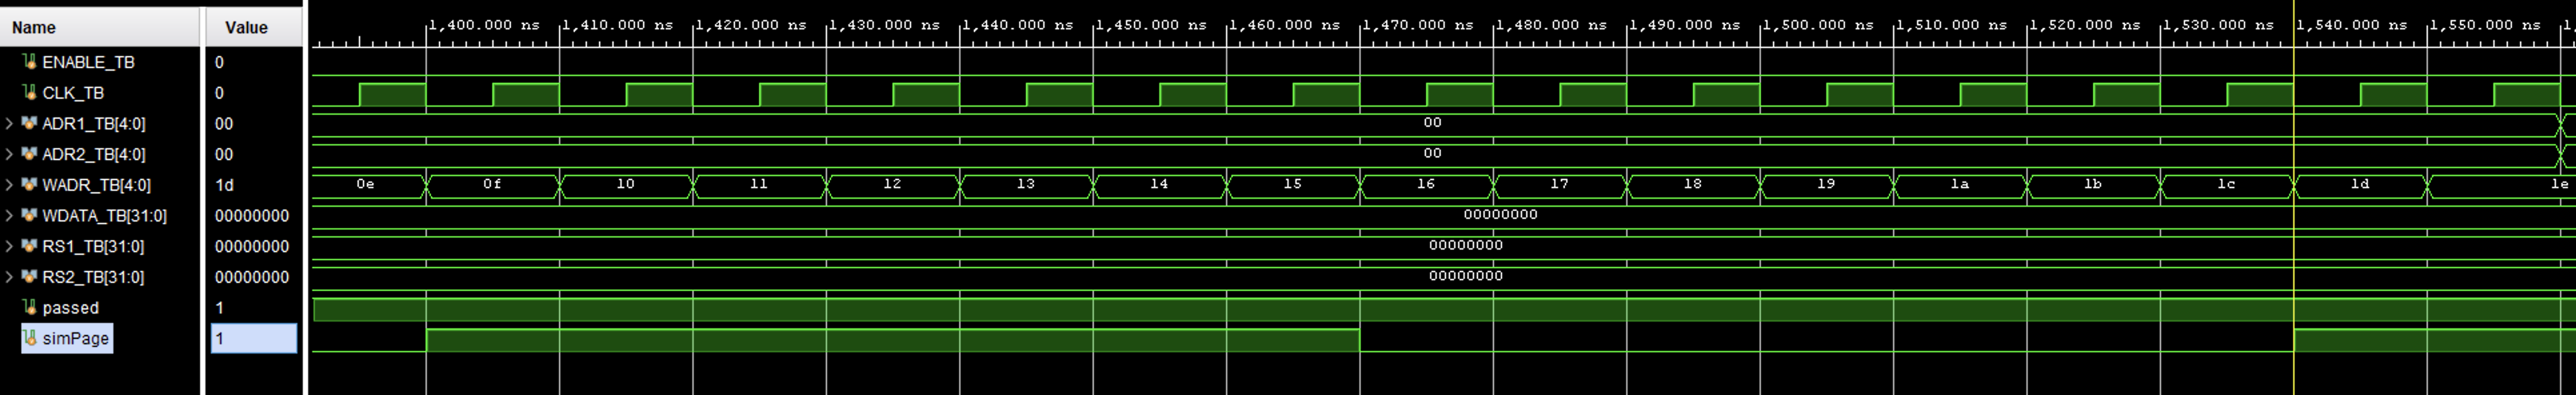
\includegraphics[width=.80\pdfpagewidth]{Figures/RegFile Simulation 10.png}
    \caption{RegFile Simulation 1400ns - 1540ns}
    \label{fig:regfilesim11}
\end{figure}

\begin{figure}[H]
    \centering
    \captionsetup{style=widetable}
    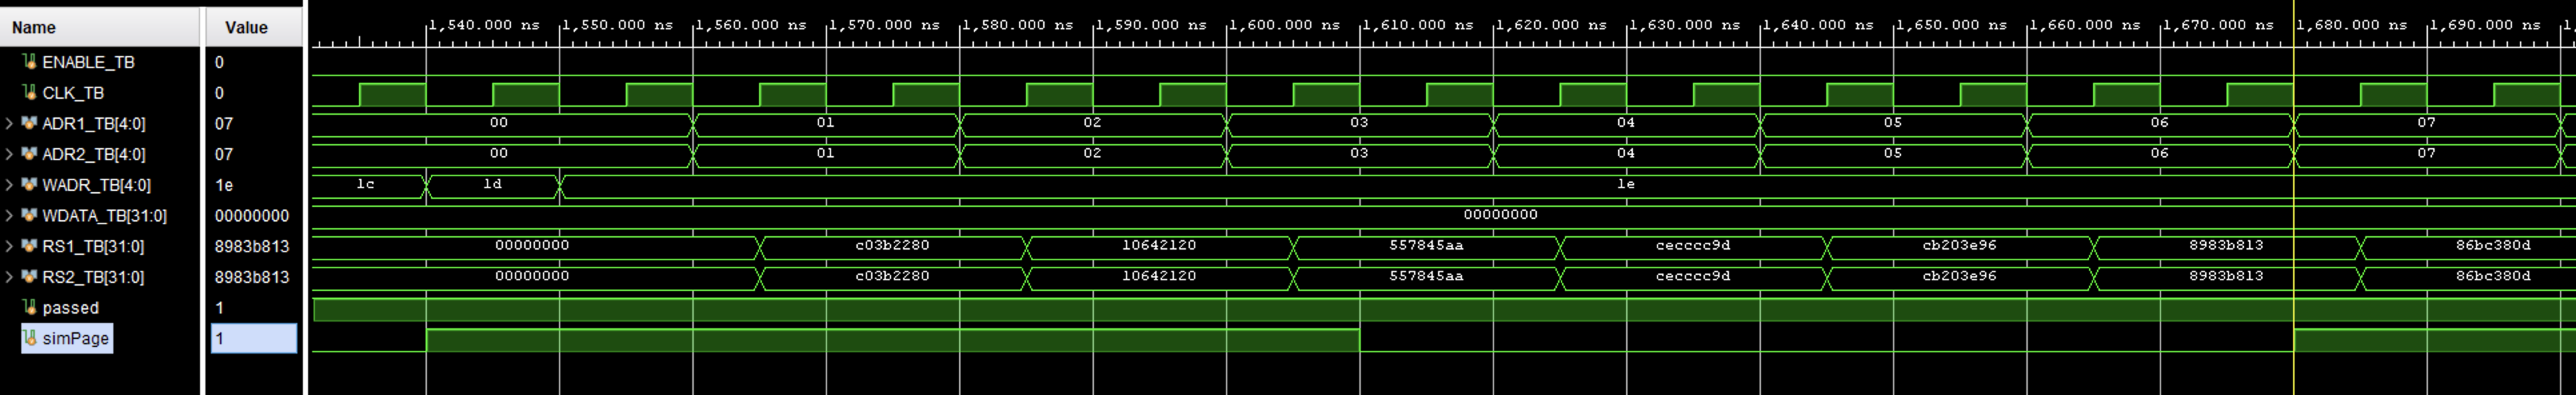
\includegraphics[width=.80\pdfpagewidth]{Figures/RegFile Simulation 11.png}
    \caption{RegFile Simulation 1540ns - 1680ns}
    \label{fig:regfilesim12}
\end{figure}

\begin{figure}[H]
    \centering
    \captionsetup{style=widetable}
    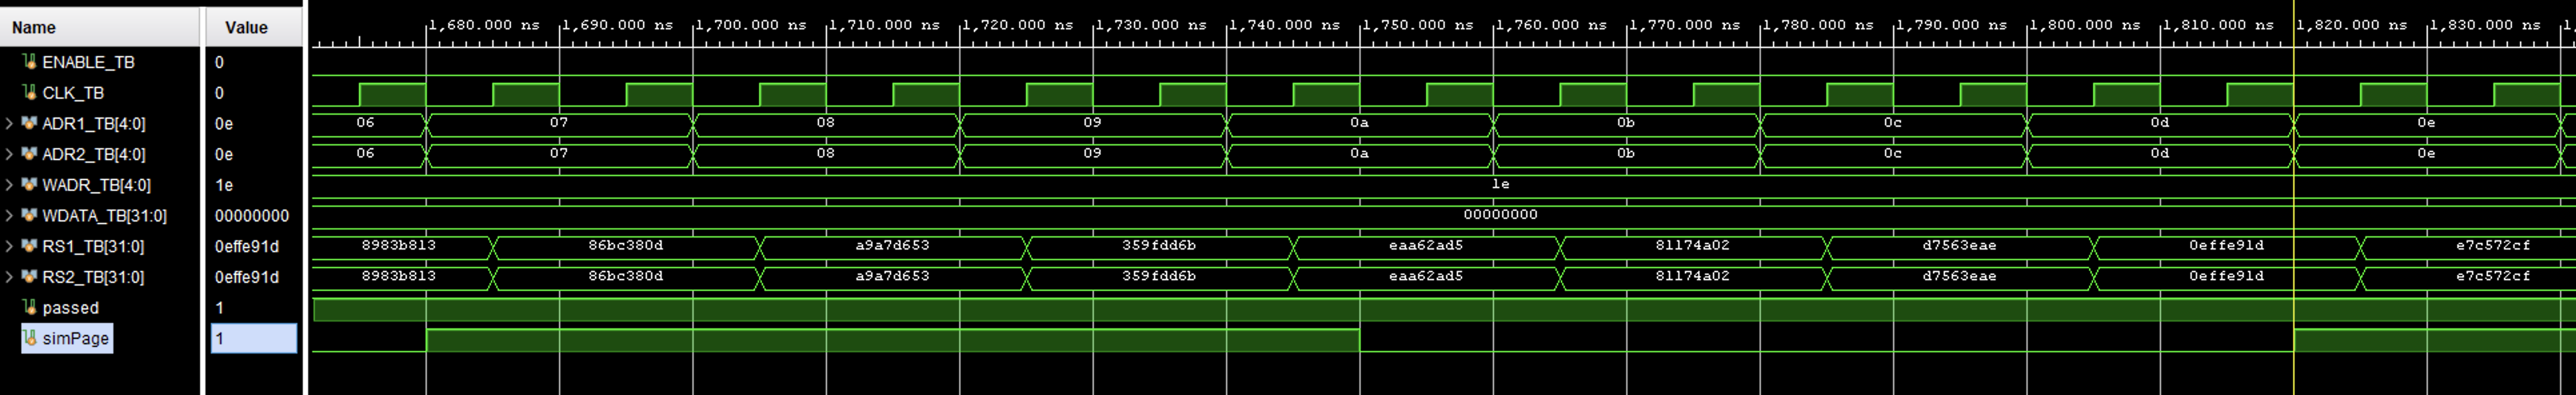
\includegraphics[width=.80\pdfpagewidth]{Figures/RegFile Simulation 12.png}
    \caption{RegFile Simulation 1680ns - 1820ns}
    \label{fig:regfilesim13}
\end{figure}

\begin{figure}[H]
    \centering
    \captionsetup{style=widetable}
    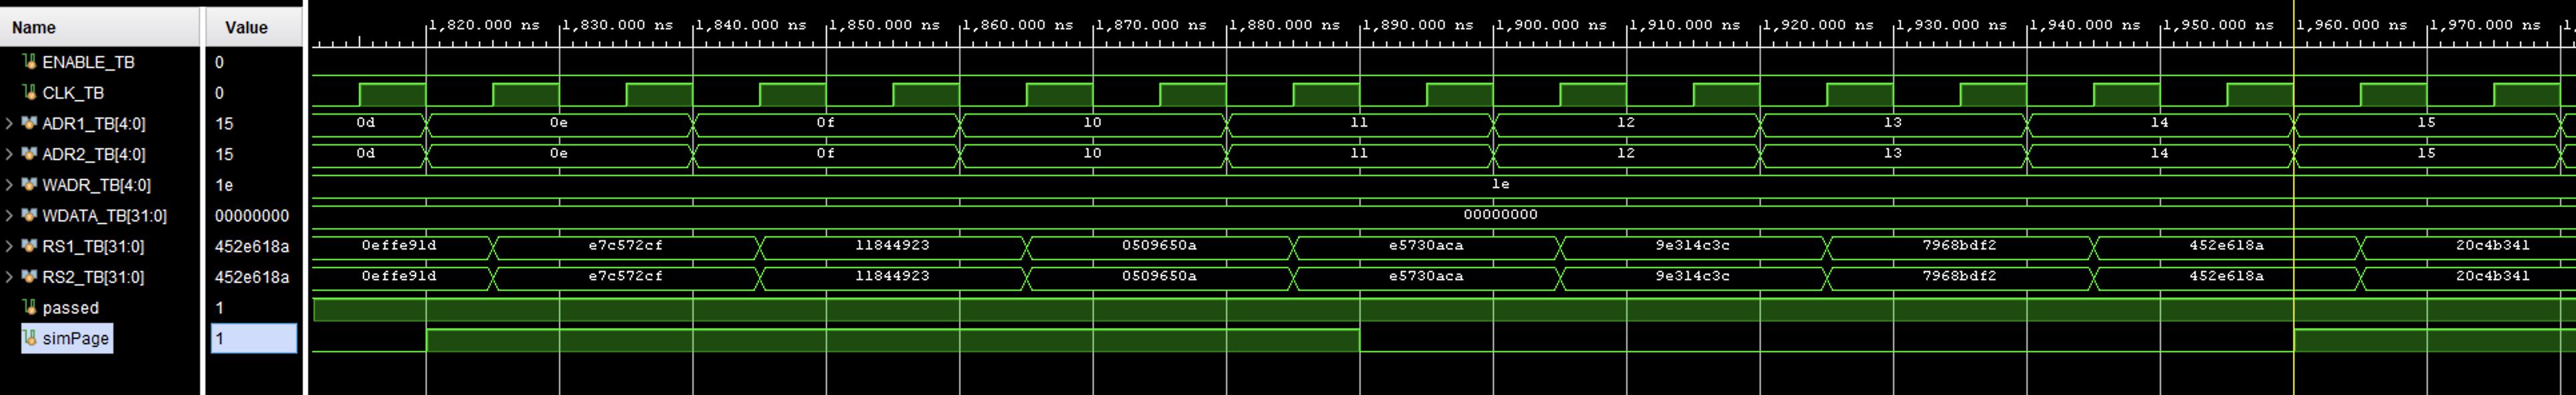
\includegraphics[width=.80\pdfpagewidth]{Figures/RegFile Simulation 13.png}
    \caption{RegFile Simulation 1820ns - 1960ns}
    \label{fig:regfilesim14}
\end{figure}

\begin{figure}[H]
    \centering
    \captionsetup{style=widetable}
    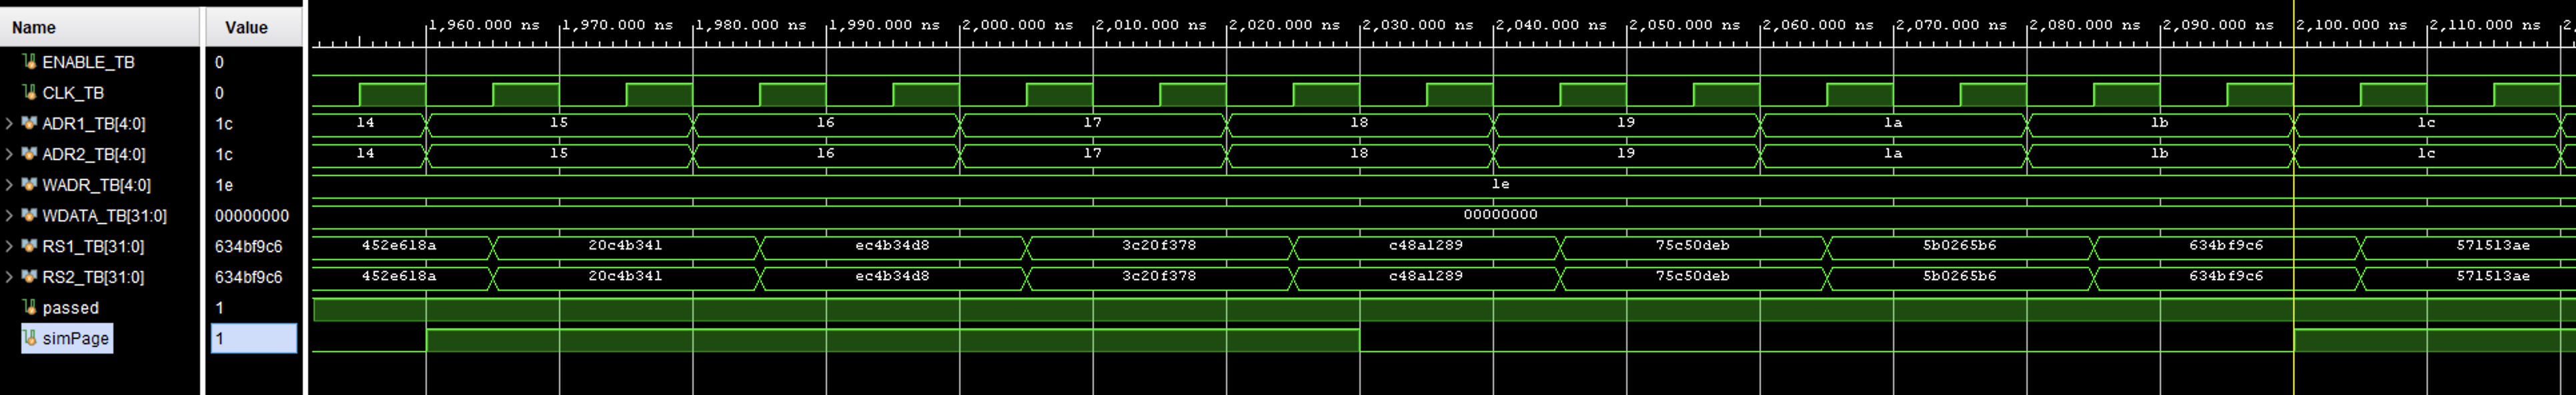
\includegraphics[width=.80\pdfpagewidth]{Figures/RegFile Simulation 14.png}
    \caption{RegFile Simulation 1960ns - 2100ns}
    \label{fig:regfilesim15}
\end{figure}

\begin{figure}
    \centering
    \captionsetup{style=widetable}
    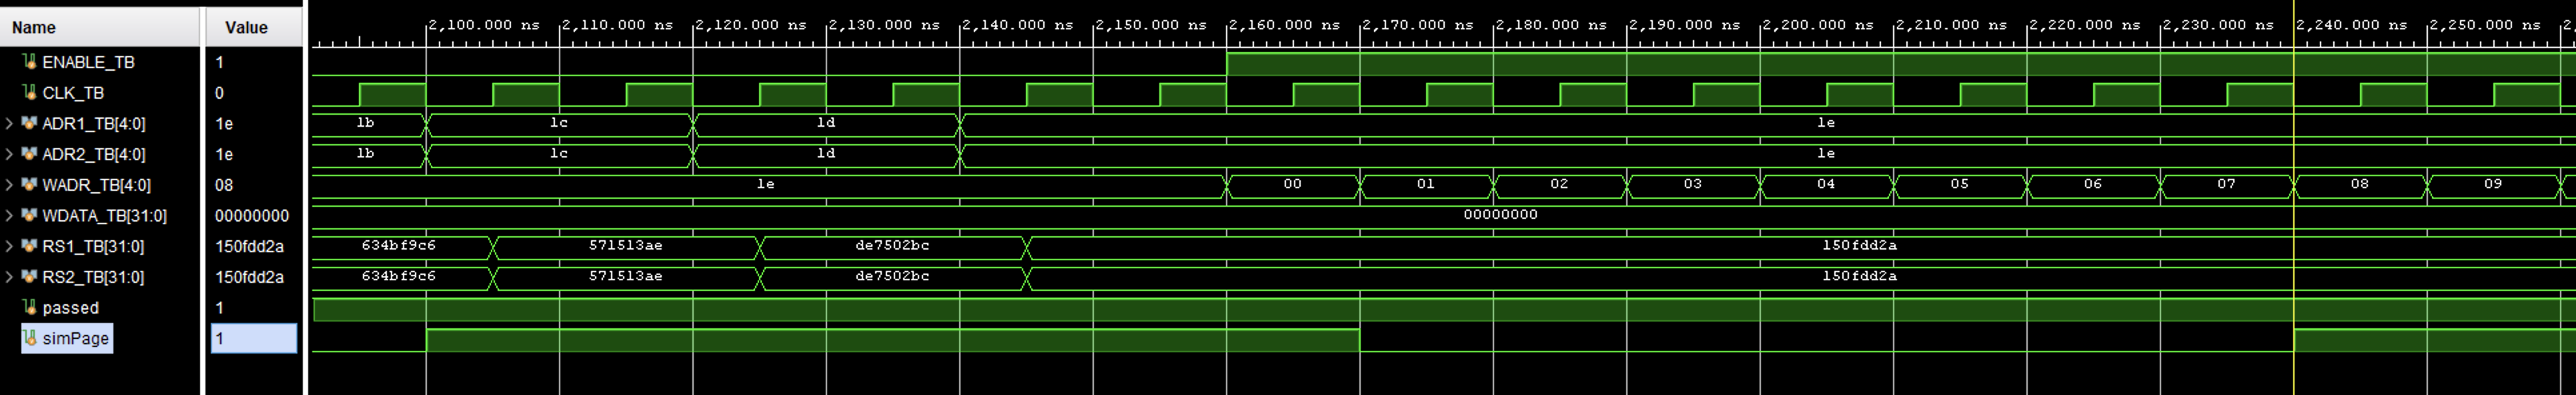
\includegraphics[width=.80\pdfpagewidth]{Figures/RegFile Simulation 15.png}
    \caption{RegFile Simulation 2100ns - 2240ns}
    \label{fig:regfilesim16}
\end{figure}

\begin{figure}
    \centering
    \captionsetup{style=widetable}
    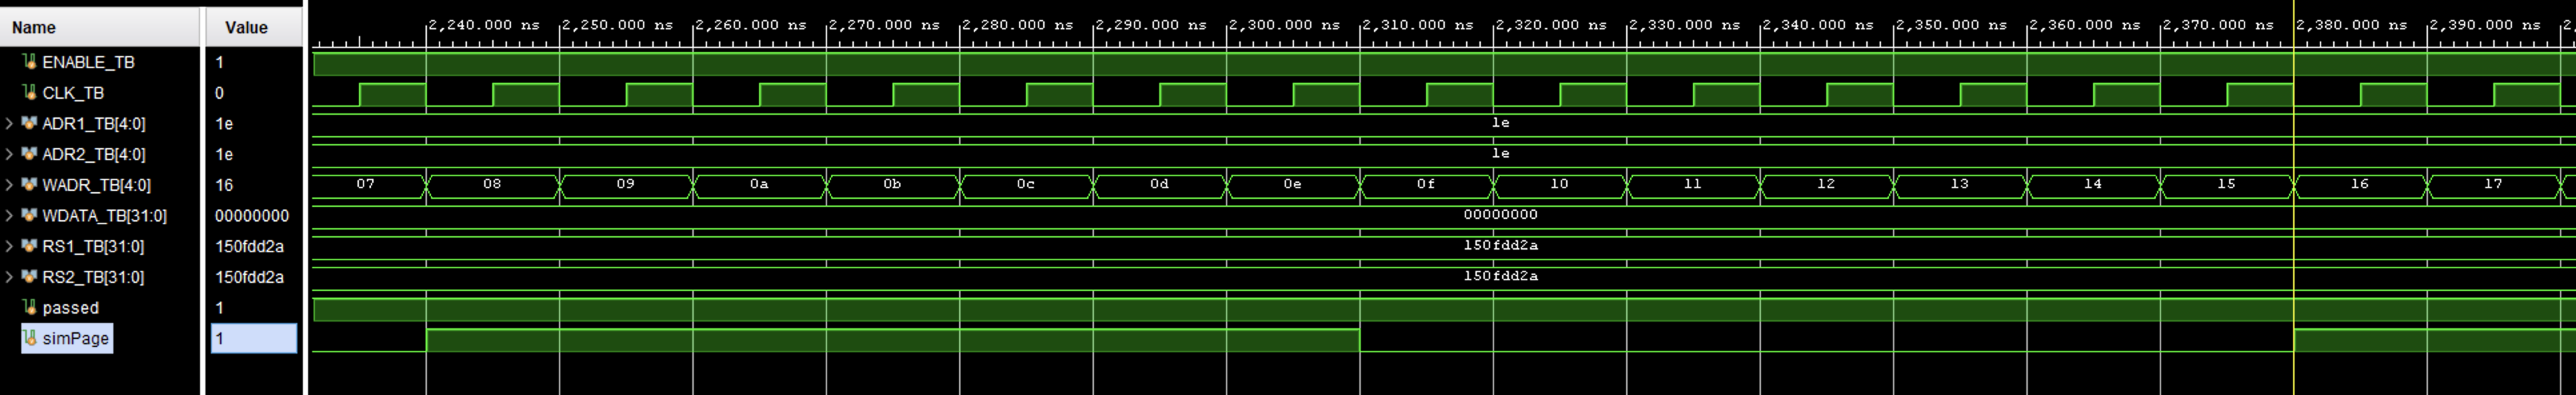
\includegraphics[width=.80\pdfpagewidth]{Figures/RegFile Simulation 16.png}
    \caption{RegFile Simulation 2240ns - 2380ns}
    \label{fig:regfilesim17}
\end{figure}

\begin{figure}
    \centering
    \captionsetup{style=widetable}
    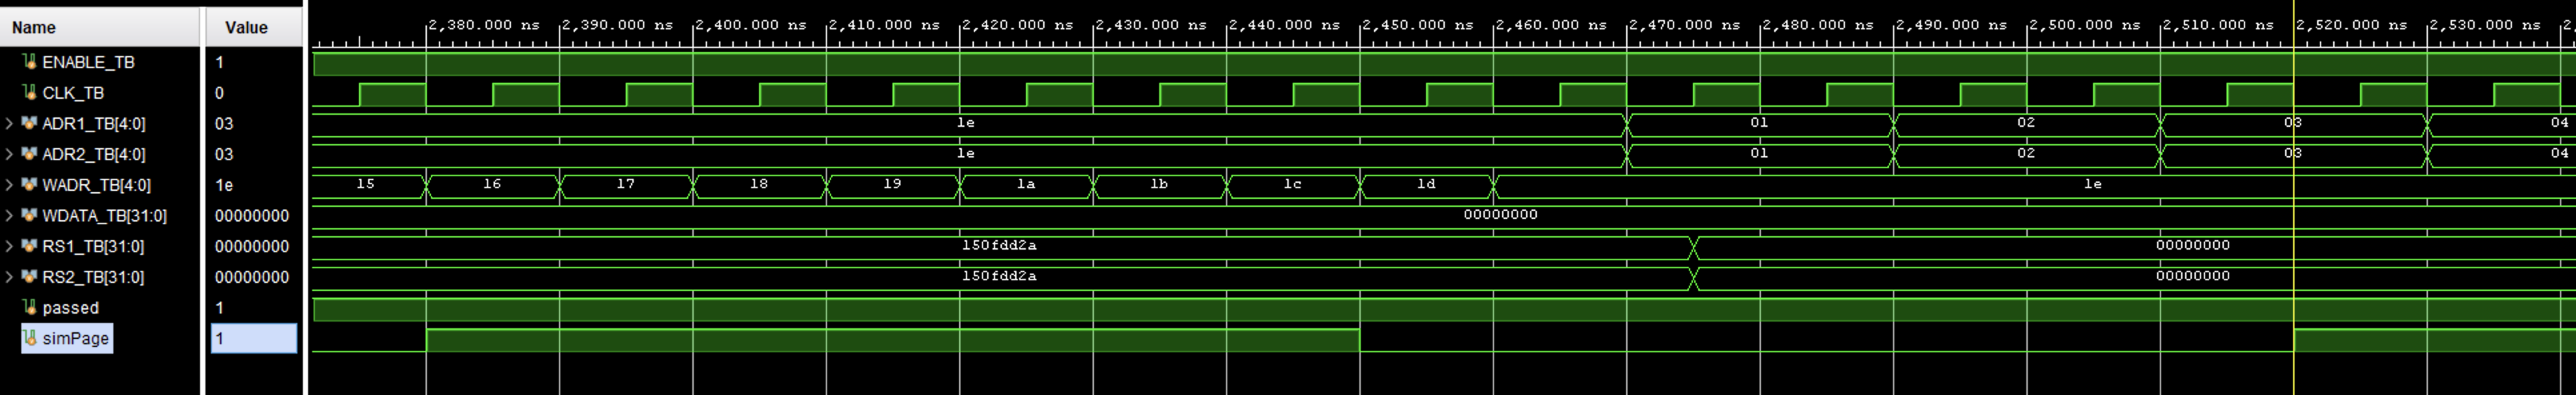
\includegraphics[width=.80\pdfpagewidth]{Figures/RegFile Simulation 17.png}
    \caption{RegFile Simulation 2380ns - 2520ns}
    \label{fig:regfilesim18}
\end{figure}

\begin{figure}
    \centering
    \captionsetup{style=widetable}
    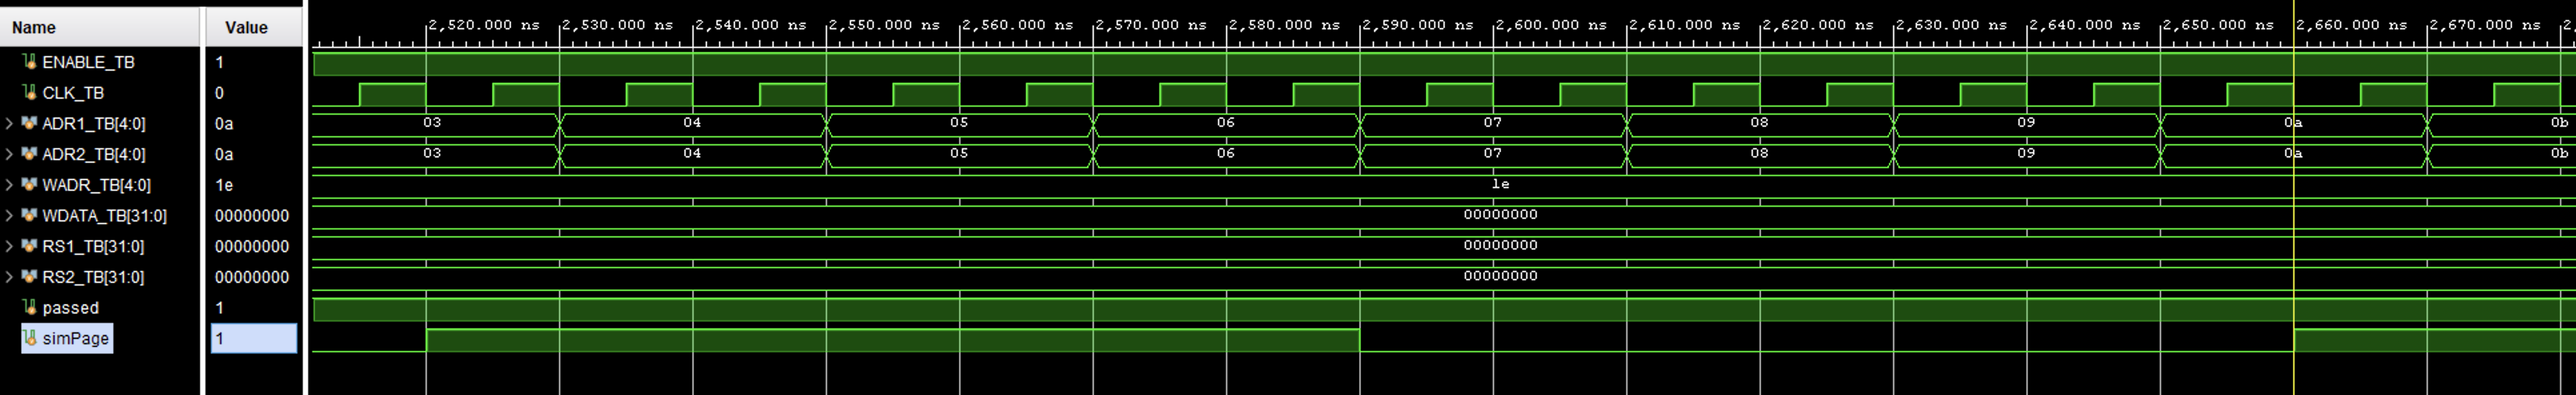
\includegraphics[width=.80\pdfpagewidth]{Figures/RegFile Simulation 18.png}
    \caption{RegFile Simulation 2520ns - 2660ns}
    \label{fig:regfilesim19}
\end{figure}

\begin{figure}
    \centering
    \captionsetup{style=widetable}
    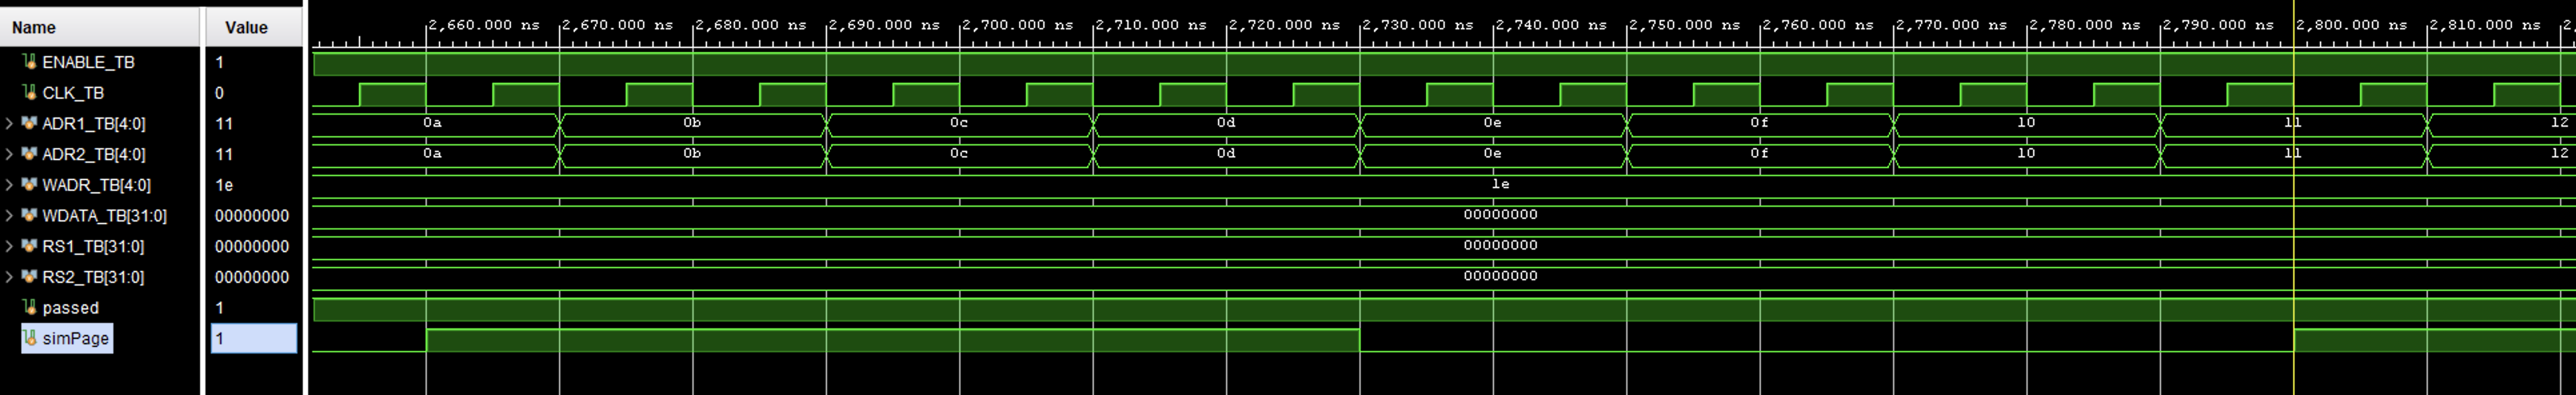
\includegraphics[width=.80\pdfpagewidth]{Figures/RegFile Simulation 19.png}
    \caption{RegFile Simulation 2660ns - 2800ns}
    \label{fig:regfilesim20}
\end{figure}

\begin{figure}
    \centering
    \captionsetup{style=widetable}
    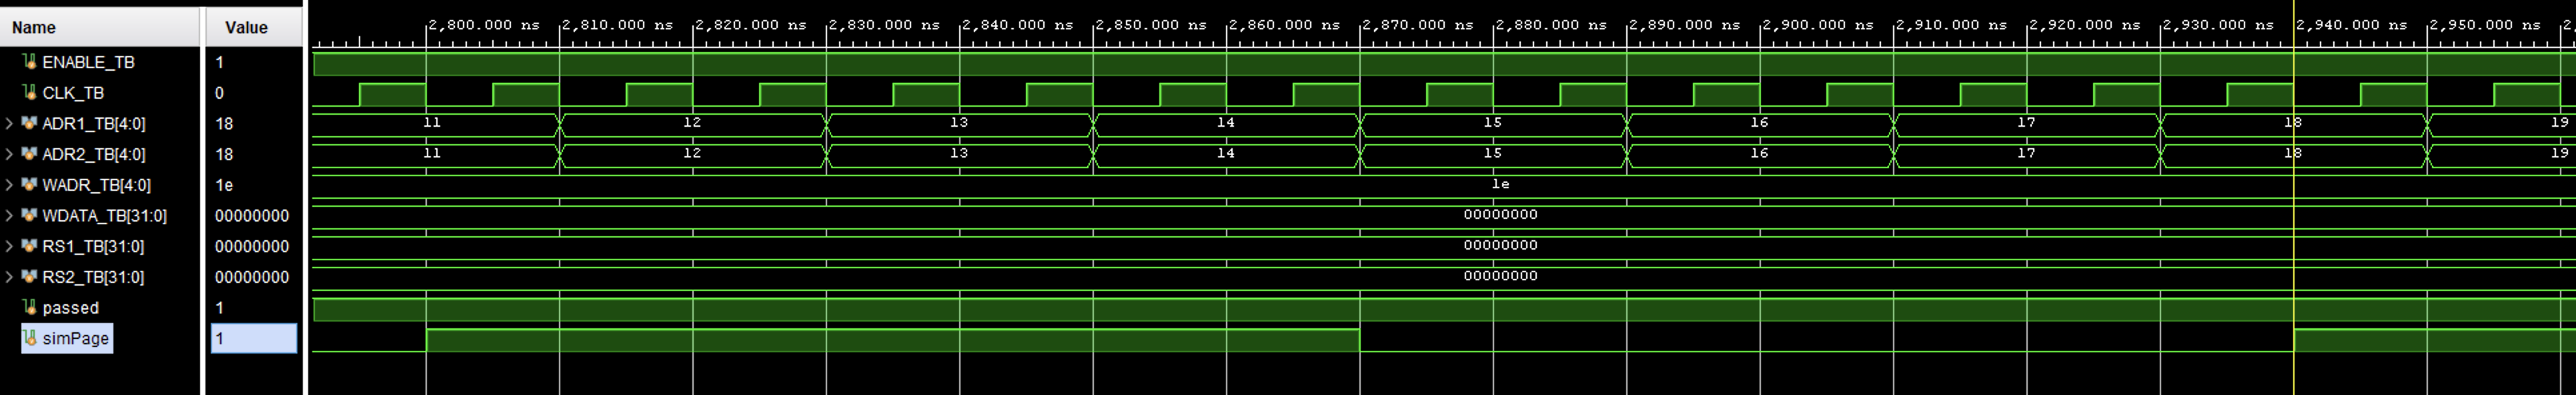
\includegraphics[width=.80\pdfpagewidth]{Figures/RegFile Simulation 20.png}
    \caption{RegFile Simulation 2800ns - 2940ns}
    \label{fig:regfilesim21}
\end{figure}

\begin{figure}
    \centering
    \captionsetup{style=widetable}
    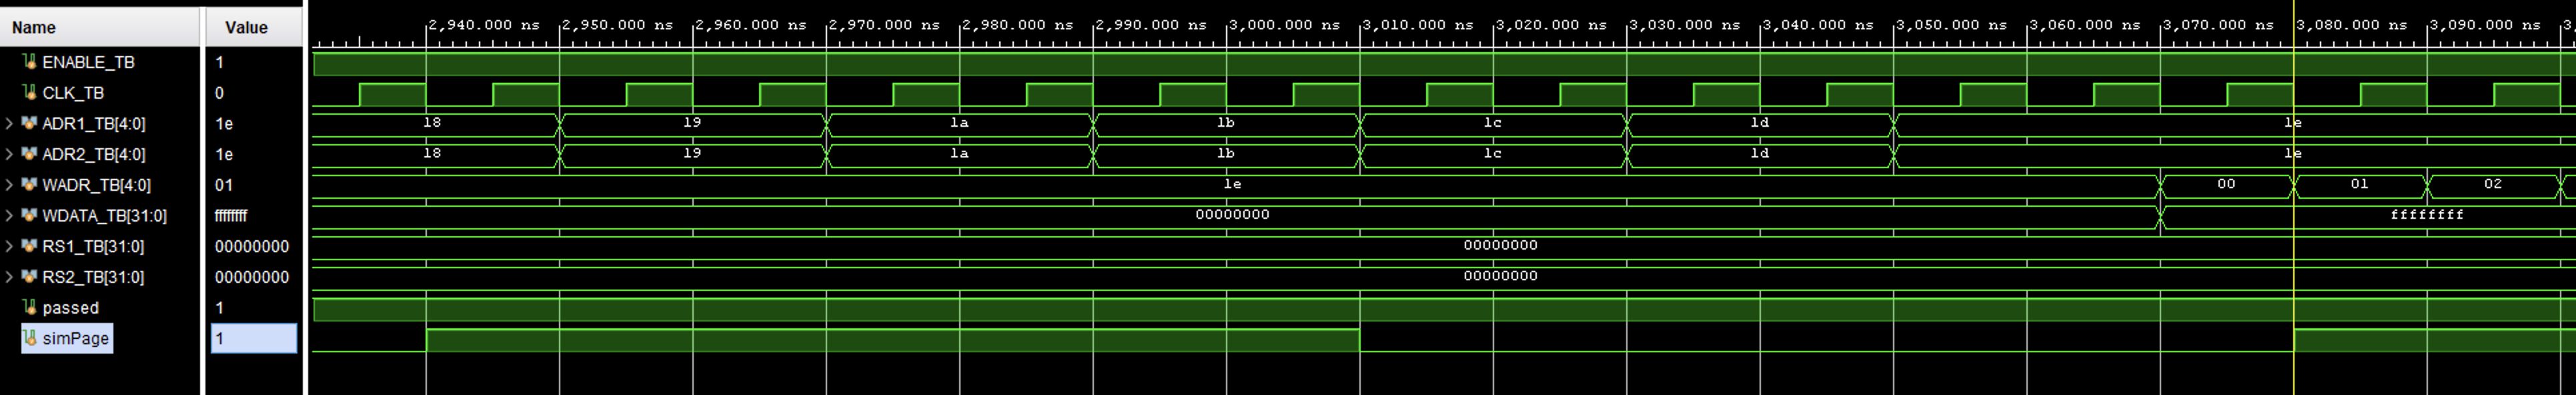
\includegraphics[width=.80\pdfpagewidth]{Figures/RegFile Simulation 21.png}
    \caption{RegFile Simulation 2940ns - 3080ns}
    \label{fig:regfilesim22}
\end{figure}

\begin{figure}
    \centering
    \captionsetup{style=widetable}
    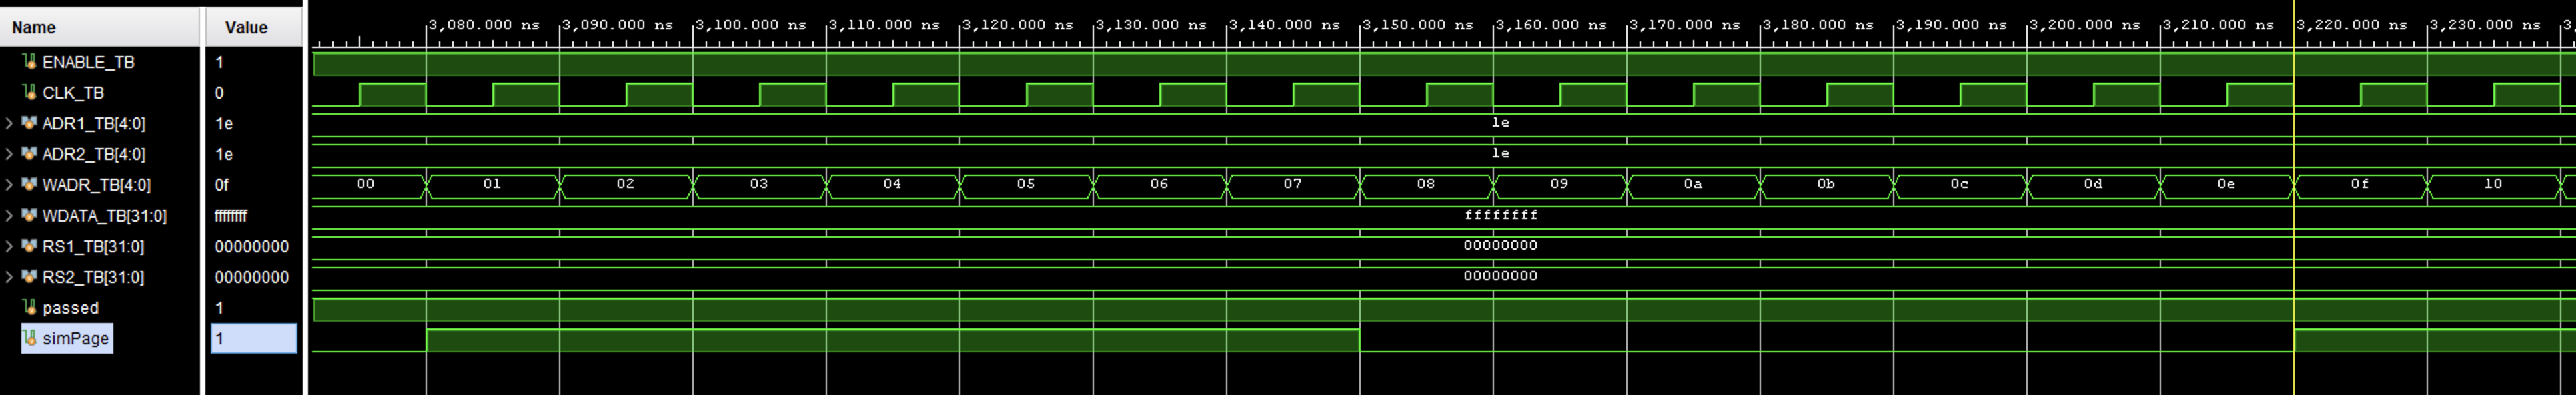
\includegraphics[width=.80\pdfpagewidth]{Figures/RegFile Simulation 22.png}
    \caption{RegFile Simulation 3080ns - 3220ns}
    \label{fig:regfilesim23}
\end{figure}

\begin{figure}
    \centering
    \captionsetup{style=widetable}
    \makebox[.80\pdfpagewidth]{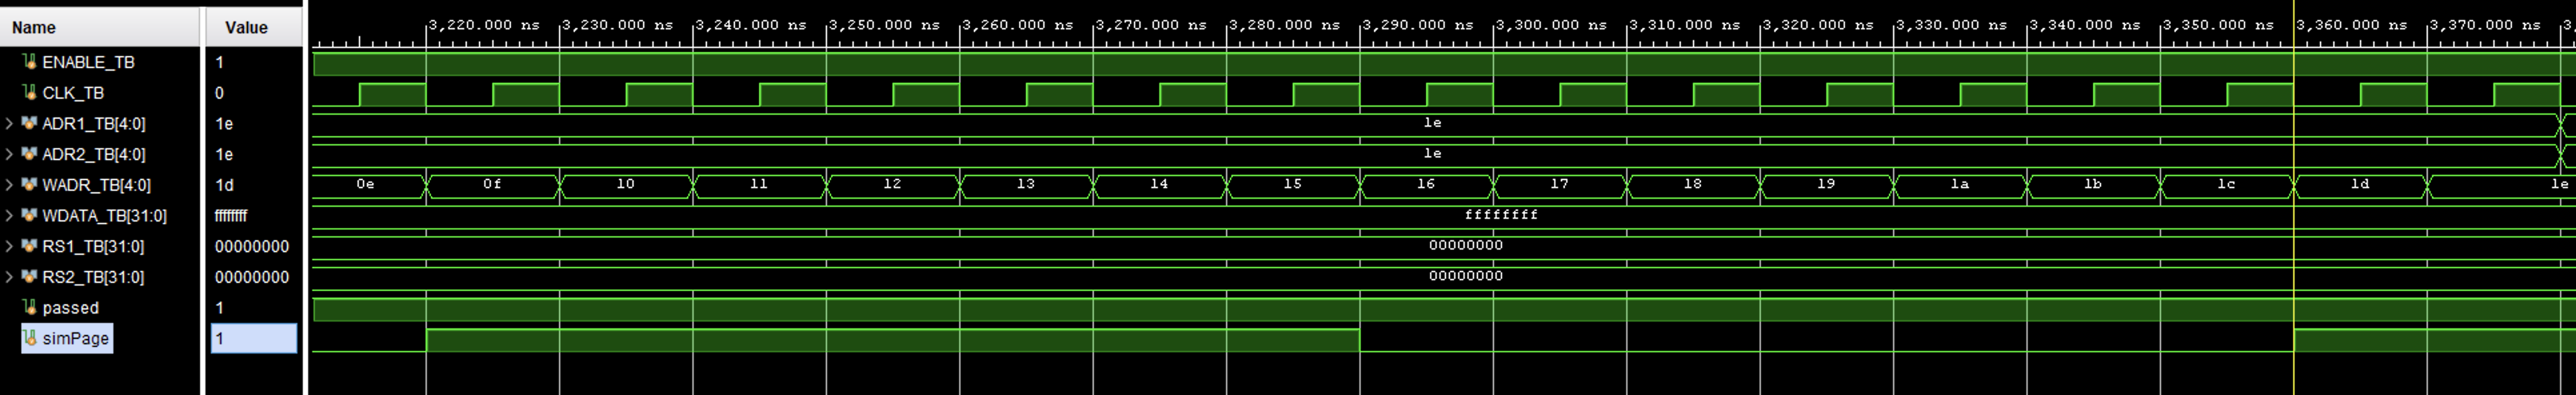
\includegraphics[width=.8\pdfpagewidth]{Figures/RegFile Simulation 23.png}}
    \caption{RegFile Simulation 3220ns - 3360ns}
    \label{fig:regfilesim24}
\end{figure}

\begin{figure}
    \centering
    \captionsetup{style=widetable}
    \makebox[.80\pdfpagewidth]{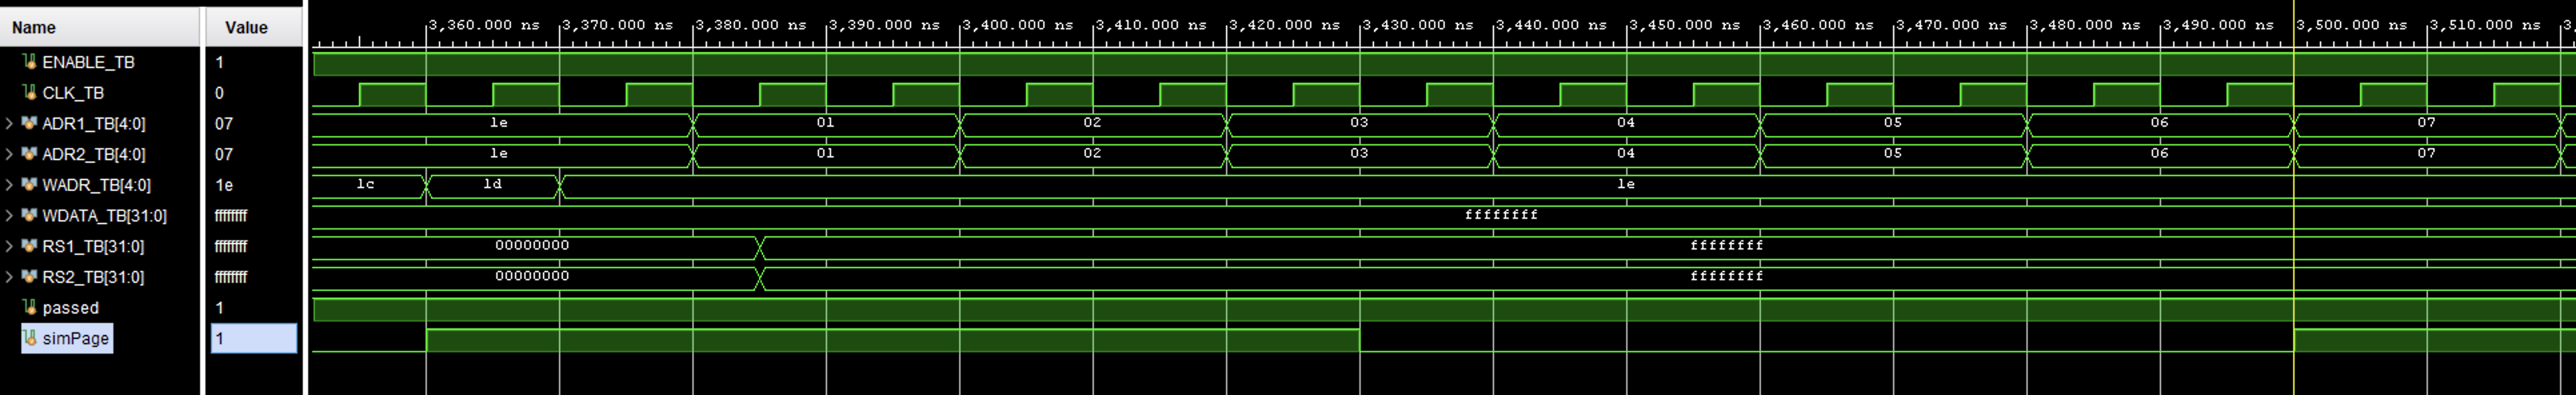
\includegraphics[width=.8\pdfpagewidth]{Figures/RegFile Simulation 24.png}}
    \caption{RegFile Simulation 3360ns - 3500ns}
    \label{fig:regfilesim25}
\end{figure}

\begin{figure}
    \centering
    \captionsetup{style=widetable}
    \makebox[.80\pdfpagewidth]{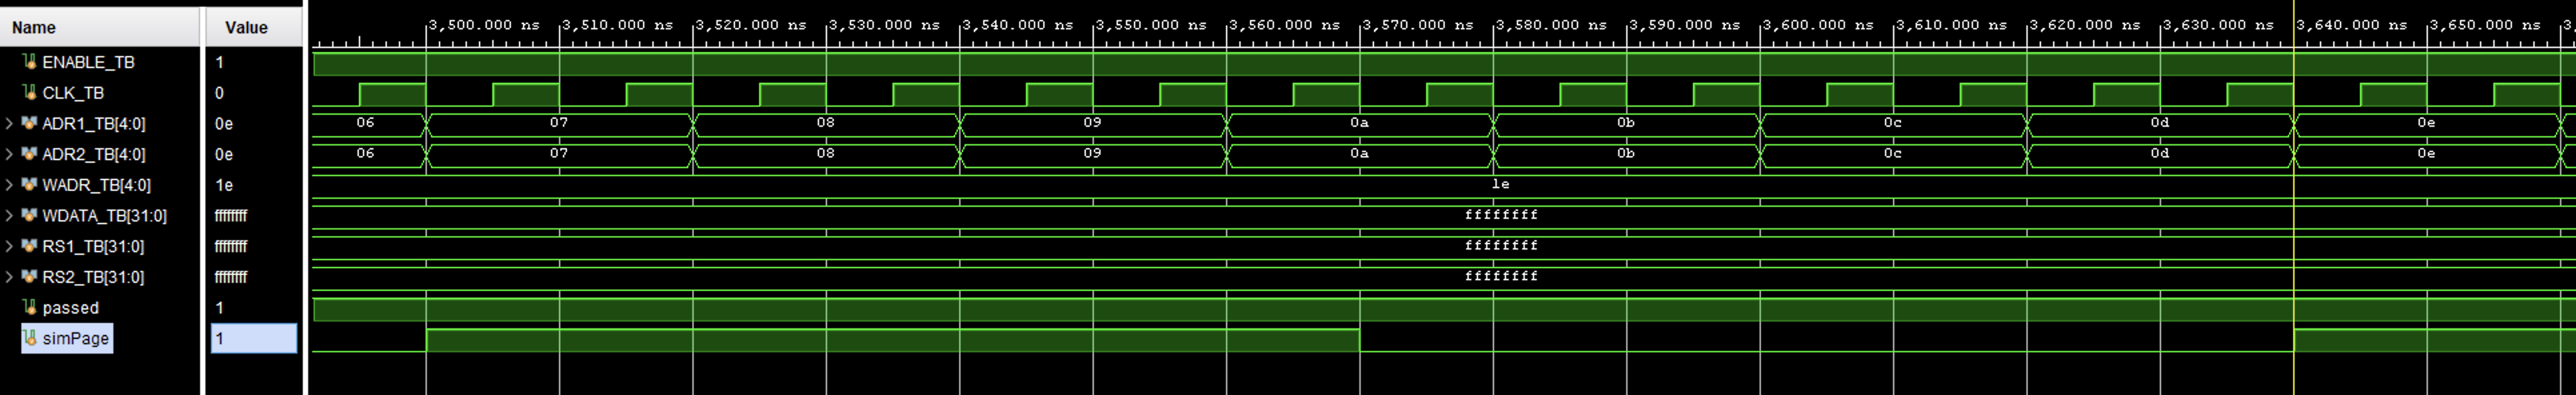
\includegraphics[width=.8\pdfpagewidth]{Figures/RegFile Simulation 25.png}}
    \caption{RegFile Simulation 3500ns - 3640ns}
    \label{fig:regfilesim26}
\end{figure}

\begin{figure}
    \centering
    \captionsetup{style=widetable}
    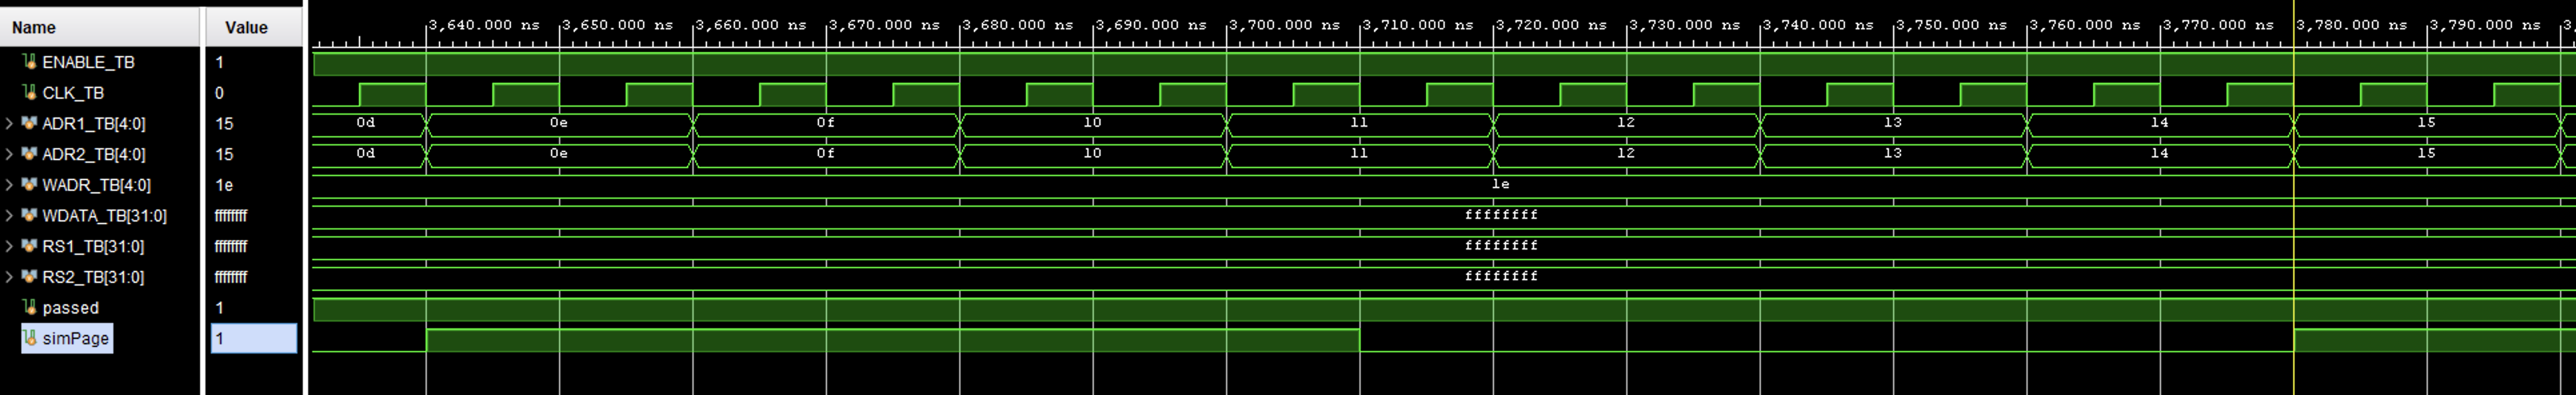
\includegraphics[width=.80\pdfpagewidth]{Figures/RegFile Simulation 26.png}
    \caption{RegFile Simulation 3640ns - 3780ns}
    \label{fig:regfilesim27}
\end{figure}

\begin{figure}
    \centering
    \captionsetup{style=widetable}
    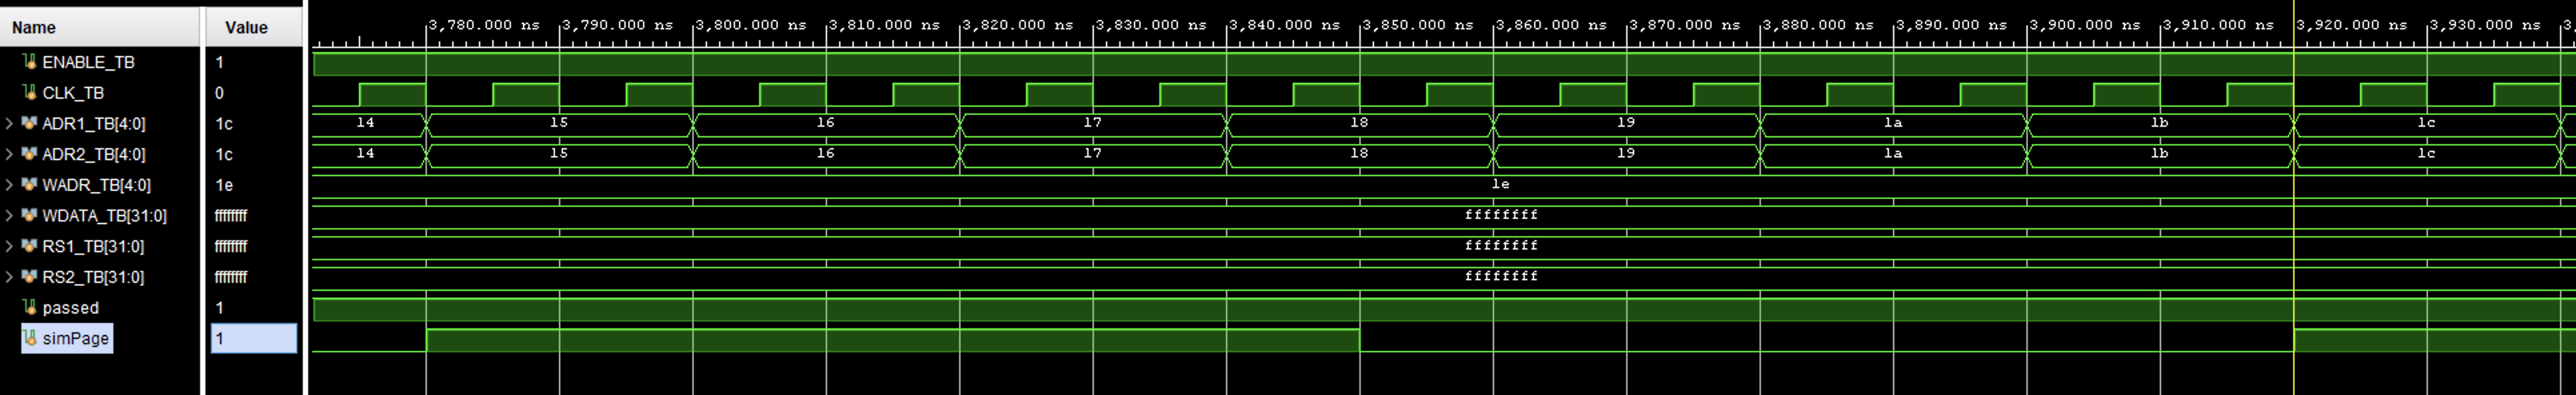
\includegraphics[width=.8\pdfpagewidth]{Figures/RegFile Simulation 27.png}
    \caption{RegFile Simulation 3780ns - 3920ns}
    \label{fig:regfilesim28}
\end{figure}


\newpage
\section{Source Code}
\captionsetup{style=widetable}
\subsection{Register File} % Third level section

\lstinputlisting[language=Verilog, caption=Verilog Code for Register File]{/Users/ethanvosburg/Documents/git/CPE-233-Otter/HW3-RegFile/RegFile/RegFile.srcs/sources_1/new/RegFile.sv}

\newpage



\section {Conclusion} % Second level section
\hypersetup{urlcolor=blue} 
The program counter is a very important module and will be used heavily in the Otter processor. This counter keeps track of which line of machine code to feed the rest of the processor and it makes allows branching and many other capabilities. In this project, a program counter was created and tested using a testbench. The testbench was able to verify that the program counter and the mux associated with it worked properly and passed all of the test cases.
All code for this assignment can be found \href{https://github.com/EthanV1920/CPE-233-Otter/tree/main}{here}.


\end{fullwidth}

\end{document}
